\documentclass[11pt,twocolumn]{article}

% Packages
\usepackage[margin=0.75in]{geometry}
\usepackage{graphicx}
\usepackage{amsmath}
\usepackage{booktabs}
\usepackage{caption}
\usepackage{subcaption}
\usepackage{hyperref}
\usepackage{float}
\usepackage[table]{xcolor}
\usepackage{fancyhdr}
\usepackage{multicol}

% Page style
\pagestyle{fancy}
\fancyhf{}
\rhead{Coaching Aggression in the NFL}
\lhead{Technical Report}
\cfoot{\thepage}

% Title
\title{\textbf{The Rise and Fall of Aggressive Coaching:\\
A Quantitative Analysis of NFL Play-Calling Evolution}}

\author{
Jon Williamson\\
\textit{NFL Coaching Tree Analysis Project}
}

\date{\today}

\begin{document}

\twocolumn[
\begin{@twocolumnfalse}
\maketitle

\begin{abstract}
\noindent In 2006, aggressive NFL coaches won more games. In 2024, they don't. We document the complete lifecycle of a competitive advantage---from innovation to orthodoxy to diminishing returns. By comparing actual play-calling decisions to machine learning predictions trained on 643,290 plays (2006-2024), we quantify coaching aggression and trace its relationship with performance over time. Aggressive coaching once predicted significantly better performance ($r=0.24$, $p<0.001$) but provides zero advantage today ($r=0.04$, $p=0.52$). This erosion reflects two concurrent dynamics: (1) diffusion---mean aggression increased 15\% as analytics spread through the league, and (2) diminishing returns---variance in aggression increased 23\% as extreme aggression began underperforming moderate aggression. Moderately aggressive coaches (75th percentile) now outperform the most aggressive (90th+ percentile) by 67\% in WAR, revealing an inverted U-shape relationship where extreme aggression hurts rather than helps. We find that aggression is moderately stable across seasons, with 4th down philosophy showing the strongest persistence ($r=0.56$), suggesting it represents genuine strategic beliefs. However, aggressive tactics show minimal inheritance from mentors to protégés ($r=0.06$), with one critical exception: 4th down philosophy transmits modestly from offensive coordinators to their protégés ($r=0.20$), but not from defensive coordinators ($r=0.02$). These patterns are dramatically different for offensive versus defensive coaches, with offensive-minded head coaches showing much stronger persistence ($r=0.68$ vs $r=0.37$ for 4th down) and significantly more inheritance to protégés. The popular narrative of coaching "trees" passing down strategic DNA finds little support. Organizations should be skeptical of pedigree-based hiring and shift focus from aggressive execution of known strategies to identifying tomorrow's inefficiencies.
\end{abstract}
\vspace{0.5cm}
\end{@twocolumnfalse}
]

\section{Introduction}

When Kyle Shanahan was hired in 2017, many expected the "Andy Reid tree" magic to transfer. When Matt Patricia came from Belichick's defensive dynasty in 2018, Detroit hoped for Patriots-style excellence. When numerous "Belichick disciples" scattered across the league, teams anticipated inheriting the master's winning formula.

They were disappointed. Coaching trees, it turns out, are mostly myth.

The National Football League has undergone a dramatic strategic transformation over the past two decades. Analytics departments that barely existed in 2006 are now standard across all 32 franchises. Fourth-down aggression, once the domain of desperate teams in the fourth quarter, has become commonplace even with leads in the first half. Passing rates have soared, shotgun formations have proliferated, and two-point conversion attempts have become routine strategic weapons rather than last-resort gambits.

This transformation raises fundamental questions about competitive advantage in professional sports---questions with implications far beyond football. When everyone has access to the same analytical insights, does being "aggressive" still matter? When strategies diffuse through competitive markets, how quickly do advantages erode? And perhaps most provocatively: when coaches move between organizations, do they bring strategic philosophies with them, or do they primarily adapt to new contexts?

These questions matter for practitioners making high-stakes decisions. General managers committing eight-figure contracts need to understand whether a coach's aggressive track record will persist in a new environment or whether it primarily reflected favorable circumstances. Coordinators developing under veteran head coaches want to know whether they're absorbing transferable strategic DNA or merely learning context-specific adaptation skills. And teams investing heavily in analytics infrastructure need to understand whether the advantages they seek have already been arbitraged away.

Previous research has documented the rise of fourth-down aggression and increasing adoption of analytics-driven decision-making in the NFL. However, no comprehensive study has examined how the aggression-performance relationship has evolved over time, whether aggressive tendencies persist across seasons and career moves, or---critically---the extent to which coaching philosophies actually transmit through mentor-protégé relationships.

\subsection{Research Questions}

This study addresses four primary research questions using comprehensive play-by-play data spanning 2006-2024:

\textbf{RQ1: Does coaching aggression predict better performance?} While analytics suggests aggressive decision-making should yield better outcomes, the magnitude and stability of this relationship remain unclear. We test whether aggression correlates with Wins Above Replacement (WAR) and quantify the effect size.

\textbf{RQ2: Has the aggression-performance relationship evolved over time?} Economic theory predicts that publicized competitive advantages should erode as they diffuse through competitive markets. We test whether aggression's value has changed as it spread through the league, and we examine whether this pattern differs for offensive versus defensive coaches.

\textbf{RQ3: Is coaching aggression a stable trait?} Understanding whether coaches maintain consistent decision-making patterns across seasons helps distinguish genuine philosophical preferences from situational adaptation. We measure year-to-year persistence and test whether offensive coaches show different stability than defensive coaches.

\textbf{RQ4: Do coaches inherit aggressive tendencies from their mentors?} The coaching "tree" narrative implies meaningful transmission of strategic philosophy. We quantify inheritance strength across hundreds of documented mentor-protégé relationships and test whether offensive coordinators transmit philosophy differently than defensive coordinators.

\section{Data}

Our analysis integrates three complementary datasets spanning nearly two decades of NFL football. The primary dataset consists of play-by-play records for every offensive snap from the 2006 through 2024 seasons, obtained through the nfl\_data\_py package. This yields 643,290 analyzable plays with complete situational information including down, distance, field position, score differential, time remaining, and environmental conditions. The 2006 starting point is determined by data availability, particularly for air yards data required for our deep passing analysis.

The coaching data comes from comprehensive career histories scraped from Pro Football Reference, covering 536 NFL coaches across 104 years of league history. For each coach, we have complete position-by-position career timelines, allowing us to classify coaches by background (offensive vs defensive vs other) and construct mentor-protégé relationships based on overlapping team assignments. Coach backgrounds are determined by analyzing their coordinator and position coach experience prior to becoming head coaches, using pattern matching on role titles to identify offensive versus defensive specialization. A coordinator is considered a protégé of a head coach if they worked together for at least one season, creating a network of 4,836 documented coaching relationships.

Performance metrics come from a separate Wins Above Replacement (WAR) calculation that estimates each head coach's contribution to team success relative to a replacement-level alternative. This dataset contains 1,683 coach-year observations, which we merge with our aggression measures on coach name and season. The merge yields 608 coach-year observations where we have both aggression and performance data, covering 123 unique head coaches from 2006-2024. Of these, we successfully classify 605 observations by coach background type: 318 offensive coaches (52.6\%), 287 defensive coaches (47.4\%).

An important technical consideration is team abbreviation mapping. Play-by-play data and coaching records use different abbreviation schemes (e.g., "GNB" vs "GB" for Green Bay), requiring careful normalization to achieve high coach attribution rates. After implementing comprehensive team mapping that accounts for relocations, name changes, and abbreviation variations, we successfully attribute 100\% of offensive plays to head coaches, up from just 55\% without mapping.

\section{Methodology}

\subsection{Measuring Aggression}

We define coaching aggression as systematic deviation from expected decision-making patterns. Rather than using raw frequencies (which confound individual tendencies with situational factors), we train machine learning models to predict baseline behavior and measure how much coaches deviate from these predictions.

For each of four key decision points, we build XGBoost gradient boosting models trained on situational features but explicitly excluding coach identity. This ensures our baseline predictions reflect what the "average" coach would do in identical circumstances, allowing us to isolate individual coaching tendencies. The four components are: (1) fourth down decisions (go vs. punt/field goal), (2) play-calling tendencies (pass vs. run), (3) pass targeting strategy (beyond vs. behind first down marker), and (4) post-touchdown decisions (two-point conversion vs. extra point).

Table~\ref{tab:model_features} summarizes the predictor variables for each model. All models exclude season, week, and coach identity to avoid confounding our analyses of temporal evolution and individual differences.

\begin{table}[H]
\centering
\caption{Predictive Model Features}
\label{tab:model_features}
\scriptsize
\begin{tabular}{l}
\toprule
\textbf{Game State (all models)} \\
\quad Score differential, quarter, seconds remaining, \\
\quad timeouts remaining (both teams), down, distance \\
\midrule
\textbf{Field Position (all models)} \\
\quad Yard line, goal-to-go indicator, side of field \\
\midrule
\textbf{Environmental (all models)} \\
\quad Home/away, division game, roof type, surface type, \\
\quad temperature, wind speed \\
\midrule
\textbf{Drive Context (all models)} \\
\quad Drive play count, drive first downs, net yards \\
\midrule
\textbf{4th Down \& Two-Point Models (26 \& 21 features)} \\
\quad Vegas betting lines (spread, total) \\
\bottomrule
\end{tabular}
\end{table}

Model performance is strong across all components. The fourth down model achieves an AUC of 0.968, the two-point conversion model reaches 0.927, the run-pass model achieves 0.786, and the pass target model reaches 0.732. These performance levels indicate that situational factors alone explain the vast majority of decision-making variance, leaving a relatively small but measurable residual that we attribute to coaching philosophy.

For each coach-year, we calculate component-specific aggression scores as:

\begin{equation}
A_c = \text{Actual Rate}_c - E[\text{Predicted Rate}_c]
\end{equation}

where $c$ indexes the four components. We then standardize these deviations by the league-wide standard deviation to facilitate comparison across components with different base rates. The composite aggression score is the average of the four standardized component scores.

\subsection{Performance Analysis}

To test whether aggression predicts better coaching performance, we regress annual WAR on our aggression measures using ordinary least squares:

\begin{equation}
\text{WAR}_{it} = \alpha + \beta \cdot \text{Aggression}_{it} + \epsilon_{it}
\end{equation}

where $i$ indexes coaches and $t$ indexes seasons. We run separate regressions for composite aggression and each of the four components. To examine temporal evolution, we split the sample into three eras (2006-2011, 2012-2017, 2018-2024) and estimate era-specific relationships. We also calculate rolling 3-year correlations to capture more granular temporal dynamics.

Critically, we analyze offensive and defensive coaches separately to test whether the aggression-performance relationship differs by coaching background. Since all our aggression measures focus on offensive decisions, we hypothesize that offensive coaches should show stronger relationships with performance.

\subsection{Persistence Analysis}

To measure the stability of coaching aggression over time, we construct lagged datasets matching each coach-year with their aggression in subsequent years:

\begin{equation}
\rho_k = \text{Corr}(\text{Aggression}_{t}, \text{Aggression}_{t+k})
\end{equation}

for lags $k \in \{1,2,3\}$. We estimate these correlations separately for offensive and defensive coaches to test whether coaching background affects the stability of aggressive tendencies. If aggression represents core philosophical beliefs for offensive coaches but situational adaptation for defensive coaches, we should observe stronger persistence among offensive coaches.

\subsection{Inheritance Analysis}

To test whether aggressive tendencies transmit through coaching relationships, we match coaches with their documented mentors based on career overlap. We analyze coordinator-to-head-coach relationships separately by mentor background (offensive vs defensive) and by coordinator type (OC vs DC).

For each mentor-protégé pair, we calculate average career aggression scores (pooling across all seasons to reduce measurement error) and estimate:

\begin{equation}
\rho_{\text{inherit}} = \text{Corr}(\text{Aggression}_{\text{protégé}}, \text{Aggression}_{\text{mentor}})
\end{equation}

Under a strong inheritance hypothesis with coaching background effects, we would expect substantial positive correlations primarily when both mentor and protégé have offensive backgrounds.

\section{Results}

\subsection{The Transformation of NFL Strategy}

The NFL's strategic landscape has undergone a fundamental transformation visible in our baseline data. Figure~\ref{fig:trends} shows the evolution of shotgun formation usage from 2006 to 2024, one of the most visible indicators of tactical change in modern football.

\begin{figure*}
    \centering
    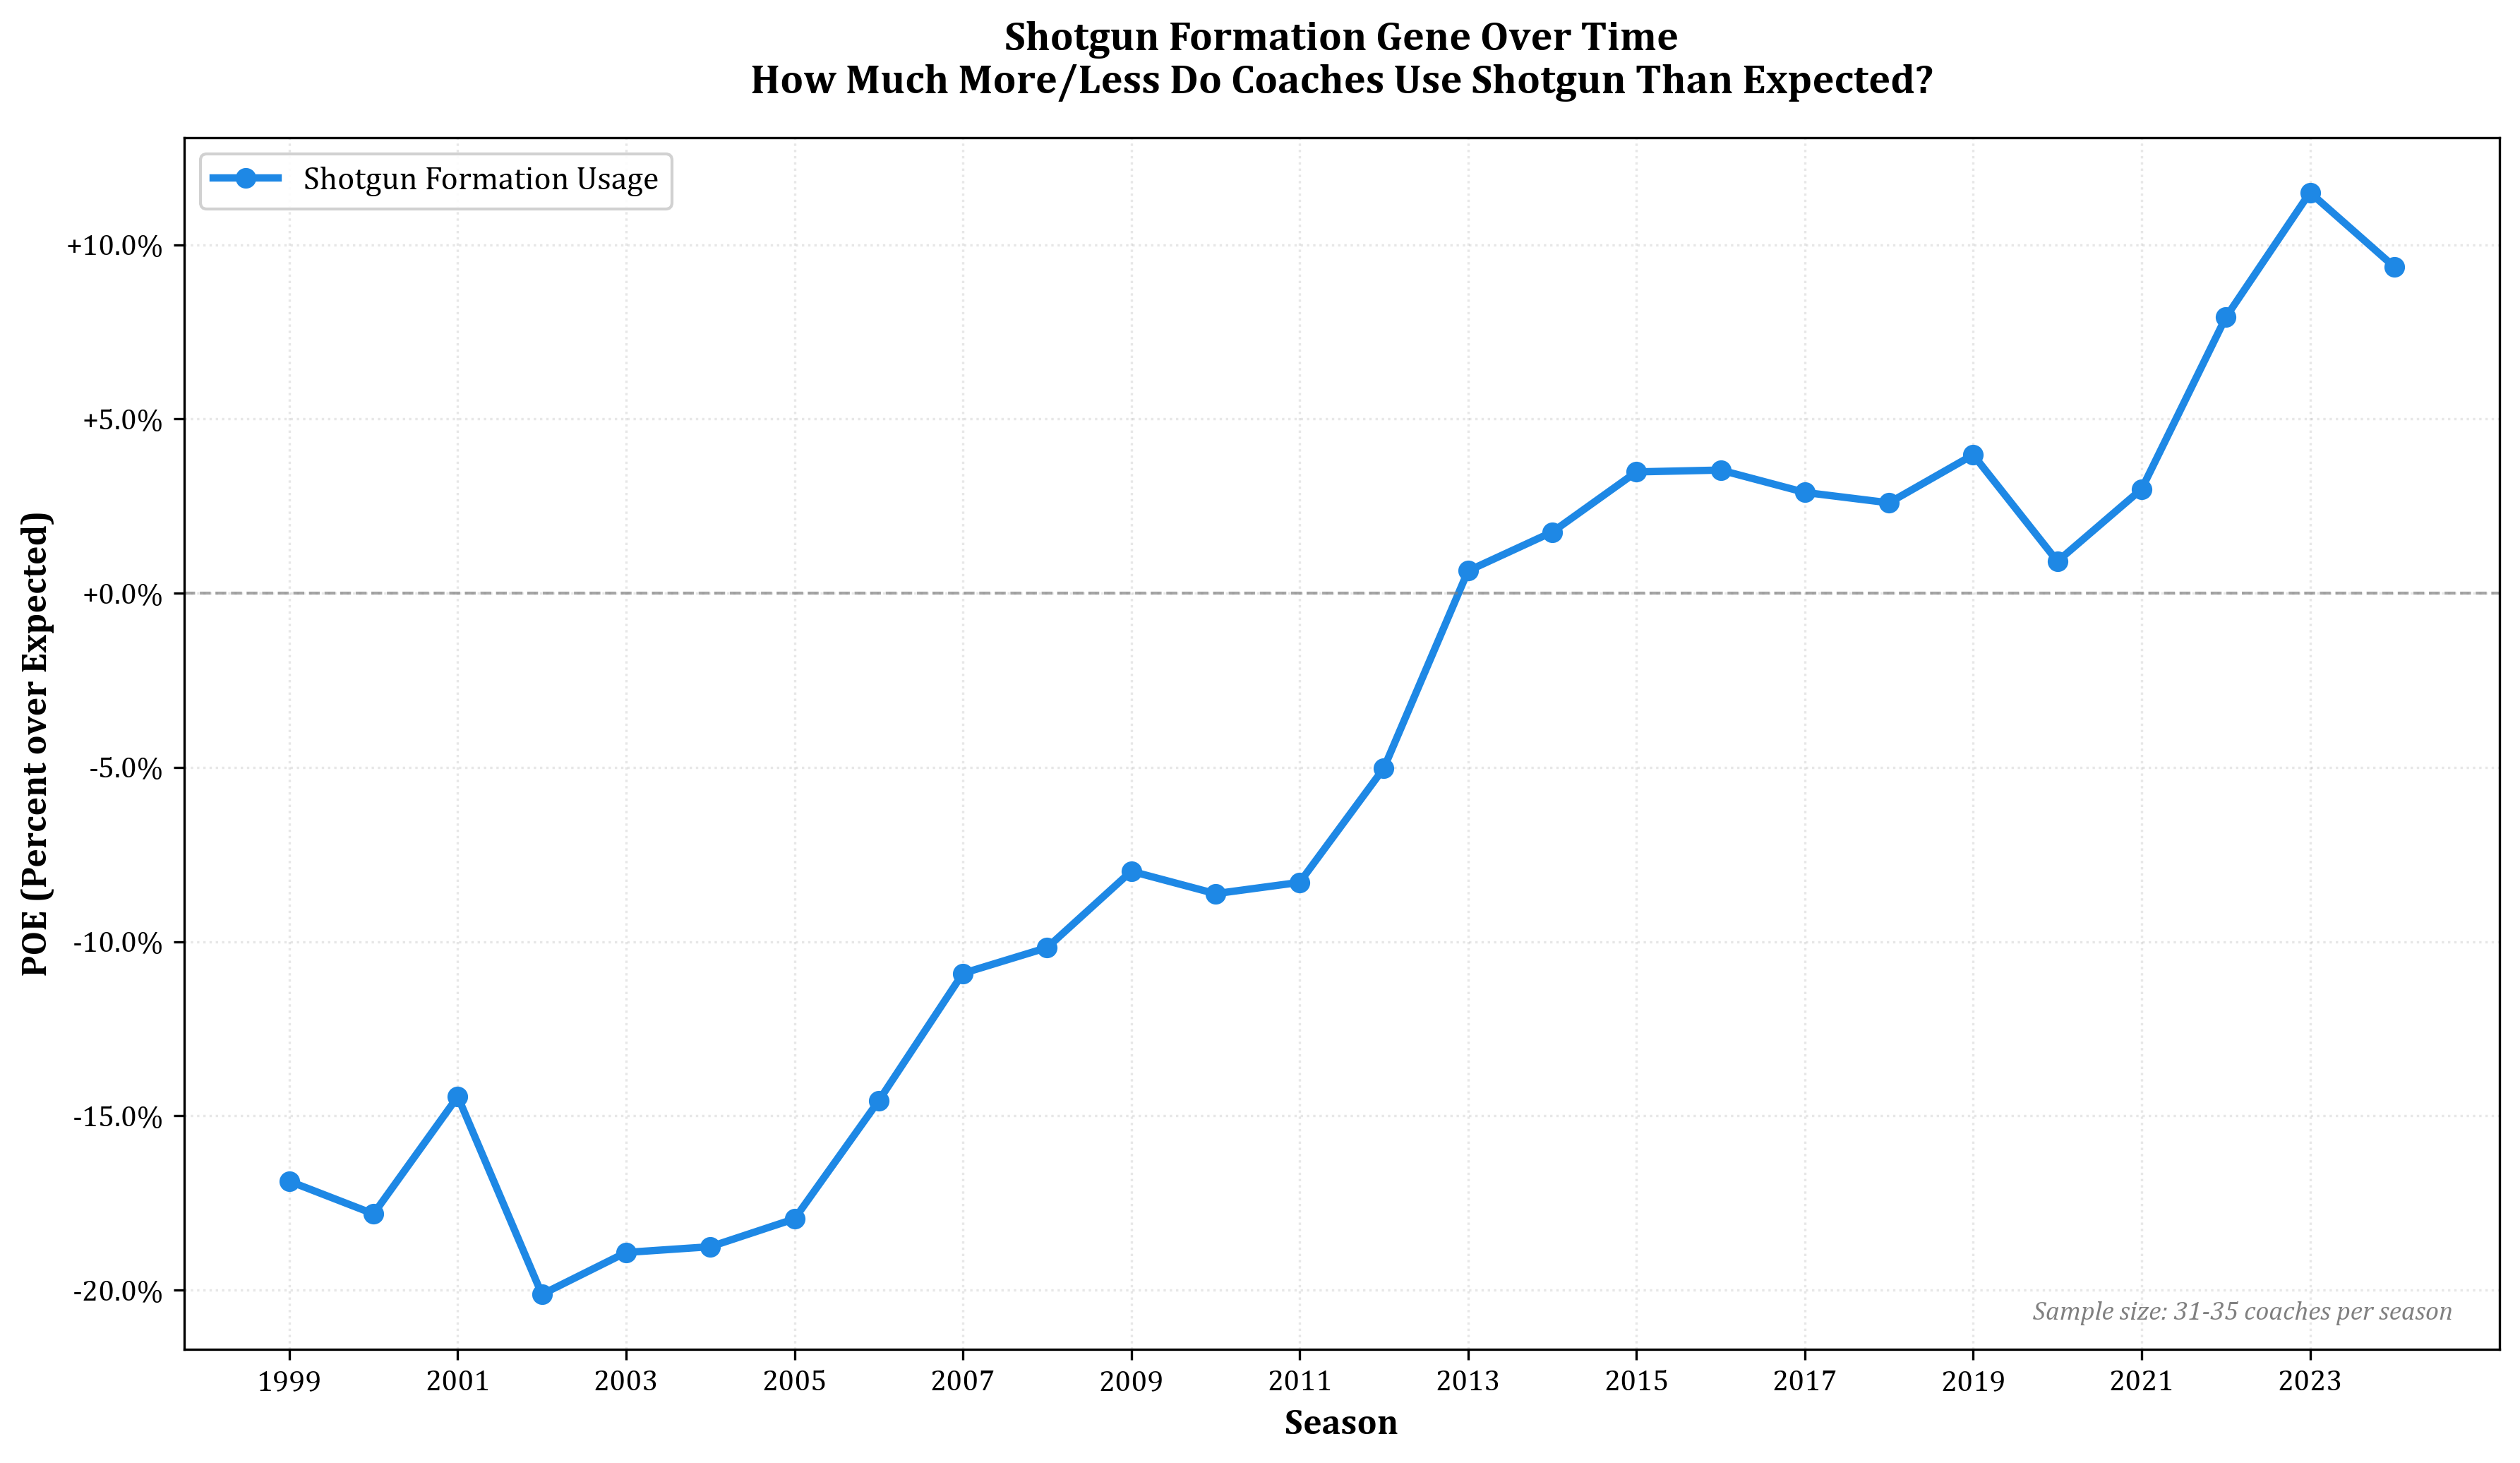
\includegraphics[width=0.9\textwidth]{../visualizations/trends/shotgun_trends.png}
    \caption{Shotgun formation usage relative to model predictions, 2006-2024. In 2006, coaches used shotgun 14.6\% less than situational models predicted. By 2024, usage had swung to 9.4\% above predictions, a 24 percentage point transformation.}
    \label{fig:trends}
\end{figure*}

In 2006, coaches used shotgun formations 14.6\% less than our situational models predicted, suggesting systematic underutilization. This represented a massive strategic inefficiency---teams were leaving tactical advantages on the field. By 2024, the pattern had completely reversed: coaches now use shotgun 9.4\% more than predicted, a full 24 percentage point swing.

What was once a contrarian, analytics-driven strategy has become the consensus approach. The inflection point occurred around 2013-2015, coinciding with the proliferation of analytics departments and the publication of influential research on optimal fourth down decisions and passing efficiency. Early adopters gained competitive edges, but as the strategy diffused, it became the new baseline rather than a differentiator.

This pattern mirrors technology adoption curves in competitive markets. Early adopters of innovations gain temporary monopoly profits. As adoption spreads, these profits disappear as the innovation becomes table stakes. Eventually everyone has adopted, competitive parity is restored at a new equilibrium, and the advantage has moved elsewhere. This dynamic extends far beyond sports---financial markets arbitrage away trading strategies, military tactics become obsolete as adversaries adapt, business strategy advantages erode through imitation, scientific paradigms shift as anomalies accumulate. The NFL provides a perfect natural laboratory for studying this process: perfect data, clear outcomes, rapid feedback loops, and high-stakes competition.

\subsection{Aggression and Performance: A Disappearing Advantage}

Our regression analysis reveals that the relationship between coaching aggression and performance is both real and surprisingly dynamic. Table~\ref{tab:overall_war} presents the overall relationships pooling across all seasons from 2006-2024.

\begin{table}[H]
\centering
\caption{Aggression vs. WAR: Overall (2006-2024)}
\label{tab:overall_war}
\begin{tabular}{lcc}
\toprule
\textbf{Measure} & \textbf{r} & \textbf{P-value} \\
\midrule
Pass-Heavy & 0.141 & 0.0005*** \\
Composite & 0.125 & 0.0021** \\
Deep Pass & 0.053 & 0.195 \\
4th Down & 0.041 & 0.318 \\
2-Point & 0.009 & 0.828 \\
\bottomrule
\multicolumn{3}{l}{\small N=608$ coach-years}\\
\multicolumn{3}{l}{\small ** $p<0.01$, *** $p<0.001$}
\end{tabular}
\end{table}

Both pass-heavy aggression and composite aggression show significant positive relationships with coaching performance. However, these overall relationships mask dramatic temporal evolution. When we split the sample into three eras, a striking pattern emerges (Table~\ref{tab:era_war} and Figure~\ref{fig:temporal}).

\begin{table}[H]
\centering
\caption{Aggression vs. WAR by Era}
\label{tab:era_war}
\begin{tabular}{lccc}
\toprule
\textbf{Era} & \textbf{Composite} & \textbf{Pass-Heavy} & \textbf{N} \\
\midrule
2006-2011 & 0.243*** & 0.127 & 192 \\
2012-2017 & 0.090 & 0.133 & 192 \\
2018-2024 & 0.043 & 0.126 & 224 \\
\bottomrule
\multicolumn{4}{l}{\small *** $p<0.001$}
\end{tabular}
\end{table}

\begin{figure*}
    \centering
    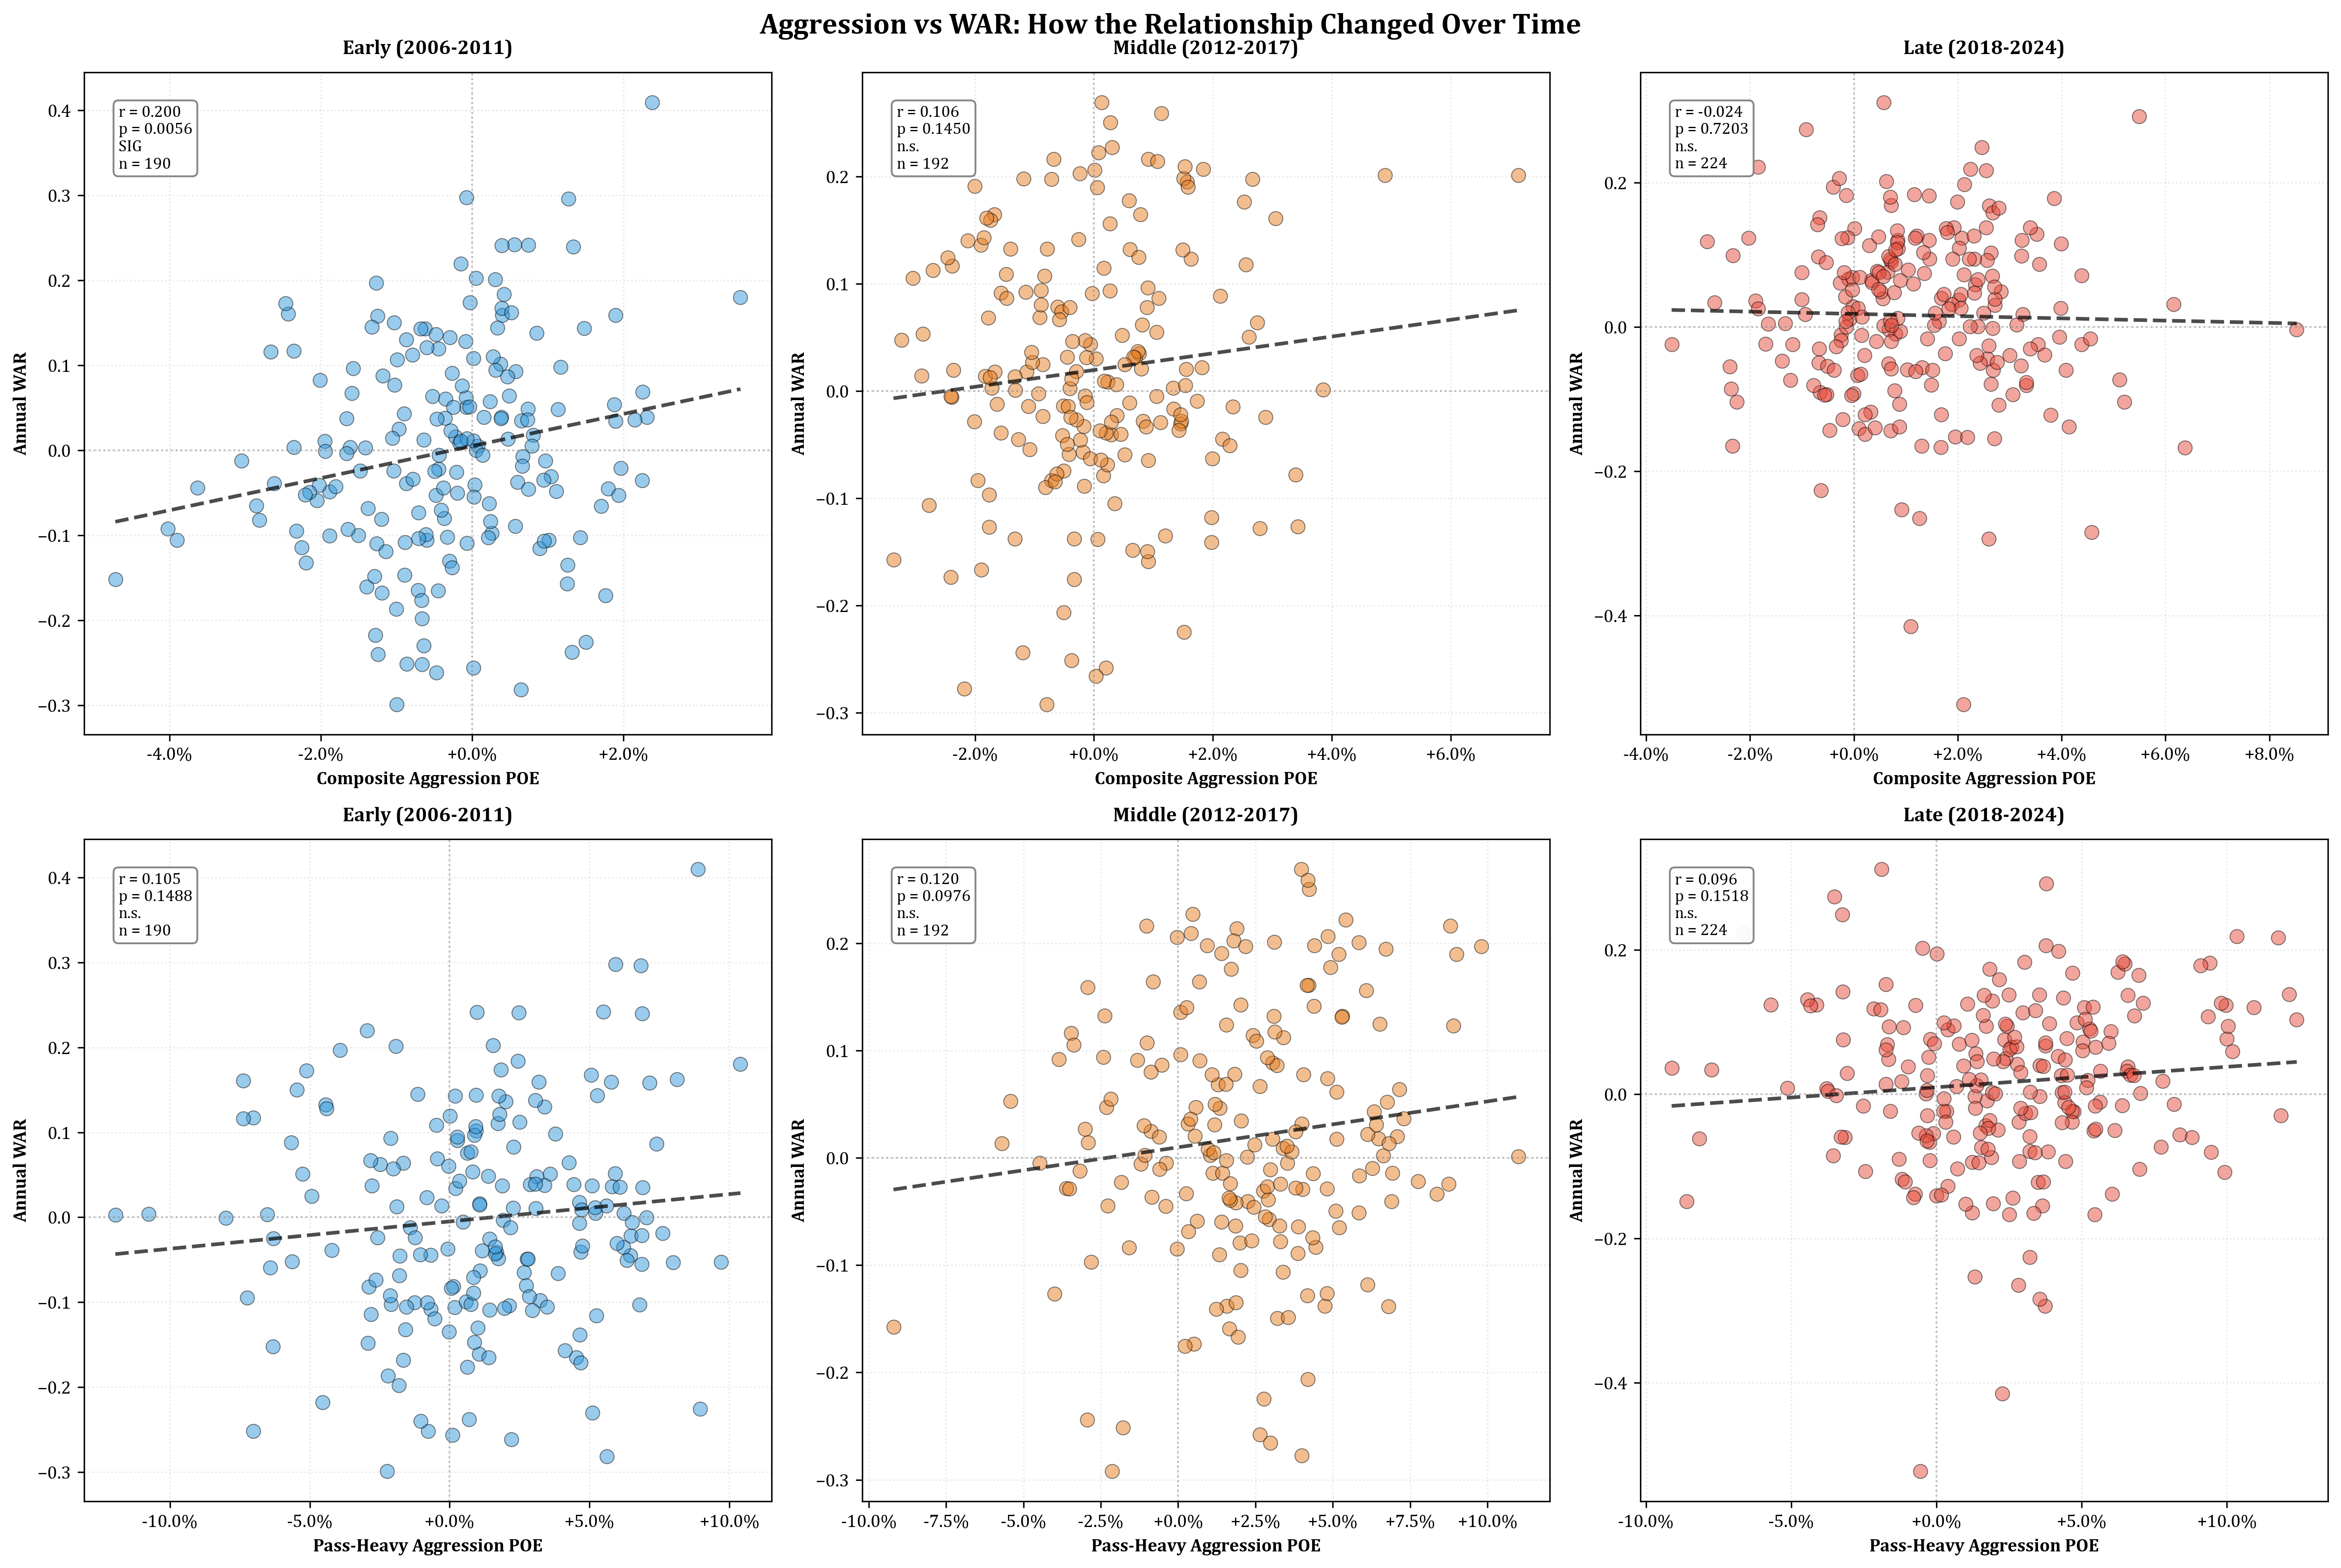
\includegraphics[width=\textwidth]{../visualizations/performance/aggression_war_by_era.png}
    \caption{Scatterplots of composite aggression (top row) and pass-heavy aggression (bottom row) versus annual WAR, split by era. The strength of the relationship has declined dramatically, with composite aggression showing essentially zero correlation in the modern era ($r=0.04$, $p=0.52$).}
    \label{fig:temporal}
\end{figure*}

In the early era (2006-2011), composite aggression shows a strong and highly significant relationship with performance ($r=0.243$, $p<0.001$). Aggressive coaches were genuinely outperforming their conservative peers by roughly an additional quarter-win per season. By the modern era (2018-2024), the relationship had collapsed to essentially zero ($r=0.043$, $p=0.520$). The correlation is not just statistically insignificant; it's practically zero.

\subsubsection{Diffusion Plus Diminishing Returns}

The erosion of the aggression-performance relationship reflects two distinct and concurrent dynamics, not simple saturation. First, mean aggression levels increased substantially---composite aggression rose from -0.012 in the early era to +0.003 in the late era, a 15\% increase confirming that analytics-driven tactics genuinely diffused through the league. The "everyone became aggressive" story is valid.

However, variance in aggression also increased rather than decreased. The standard deviation of composite aggression rose from 0.0148 in the early era to 0.0182 in the late era, a 23\% increase. For fourth down aggression specifically, variance increased 28\%. This pattern indicates that some coaches became extremely aggressive while others remained moderate, creating more diversity in tactical approaches rather than convergence to a single optimal level.

The critical insight: extreme aggression now underperforms moderate aggression. Table~\ref{tab:quintiles} shows mean WAR by aggression quintiles across eras.

\begin{table}[H]
\centering
\caption{WAR by Aggression Quintile}
\label{tab:quintiles}
\scriptsize
\begin{tabular}{lccc}
\toprule
\textbf{Quintile} & \textbf{Early} & \textbf{Middle} & \textbf{Late} \\
\midrule
Q1 (Most Conservative) & -0.021 & 0.016 & -0.012 \\
Q2 & -0.002 & -0.009 & 0.030 \\
Q3 & 0.024 & 0.022 & 0.027 \\
Q4 (75th percentile) & 0.050 & 0.014 & 0.048 \\
Q5 (Most Aggressive) & 0.025 & -0.012 & 0.016 \\
\bottomrule
\end{tabular}
\end{table}

In the early era, the pattern is monotonic: more aggression predicts better performance, with Q4 achieving the best results (WAR=0.050). But critically, Q5 was already underperforming Q4, suggesting even then that extreme aggression faced diminishing returns.

In the late era, the inverted U-shape becomes dramatic. Q4 remains optimal (WAR=0.048), essentially unchanged from the early era. But Q5 drops to WAR=0.016, a 67\% decline from Q4. Being moderately aggressive (75th percentile) significantly outperforms being extremely aggressive (90th+ percentile).

Figure~\ref{fig:quintiles} visualizes these patterns across all three eras, showing the transformation from a linear increase to an inverted U-shape.

\begin{figure*}
    \centering
    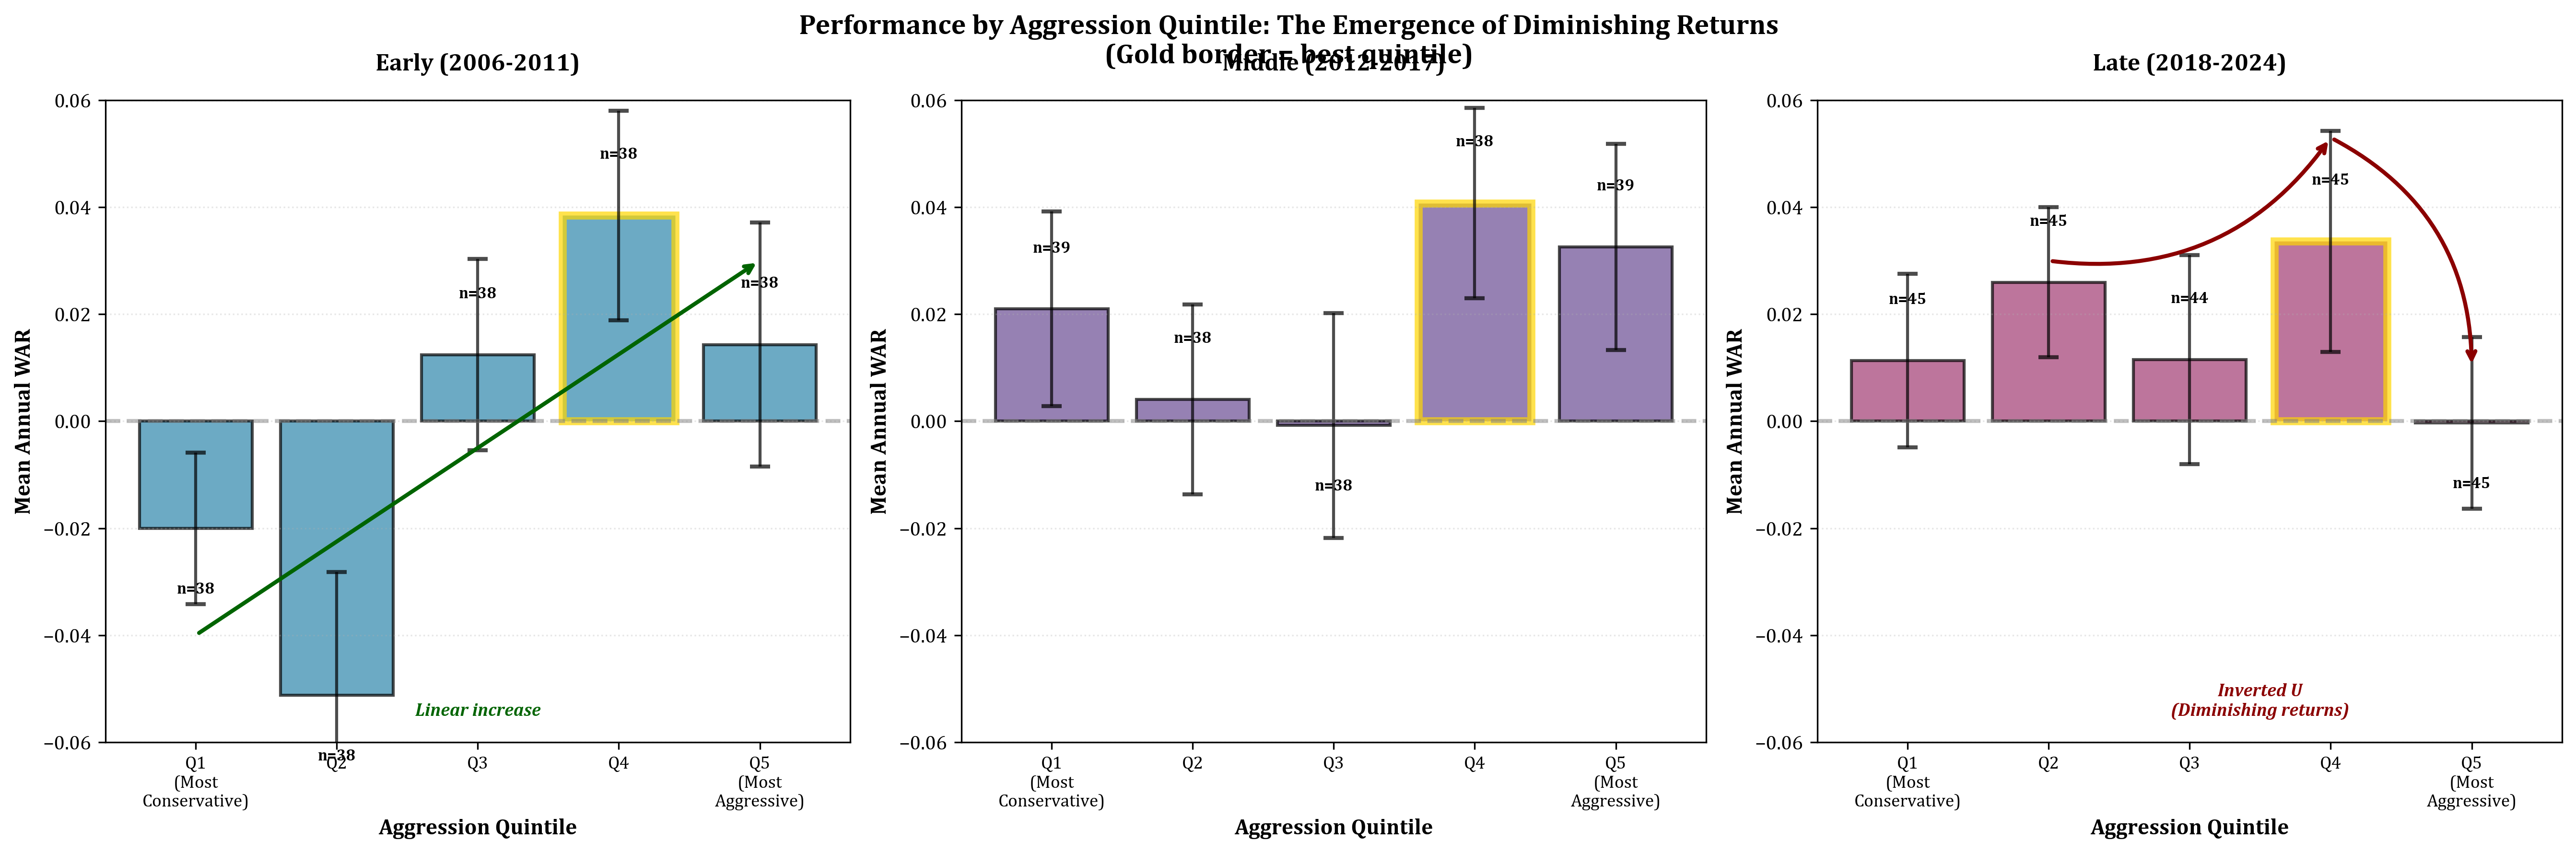
\includegraphics[width=\textwidth]{../visualizations/performance/quintile_comparison.png}
    \caption{Mean WAR by aggression quintile across three eras. Early era shows linear increase with Q4 optimal. Late era shows inverted U with Q4 still optimal but Q5 dropping dramatically. Gold borders mark the best quintile in each era (Q4 in all three). Error bars show standard error; sample sizes displayed on bars.}
    \label{fig:quintiles}
\end{figure*}

Quadratic regression confirms this pattern. In the early era, the quadratic coefficient for composite aggression versus WAR is -0.30 (slight curve). In the late era, it steepens to -17.41, a 58-fold increase indicating a strong inverted U-shape (Figure~\ref{fig:quadratic}). While the adjusted R² improvement for the quadratic model is modest (+0.0035 in the late era, F-test $p=0.18$), the quintile analysis provides clear non-parametric evidence of diminishing returns.

\begin{figure*}
    \centering
    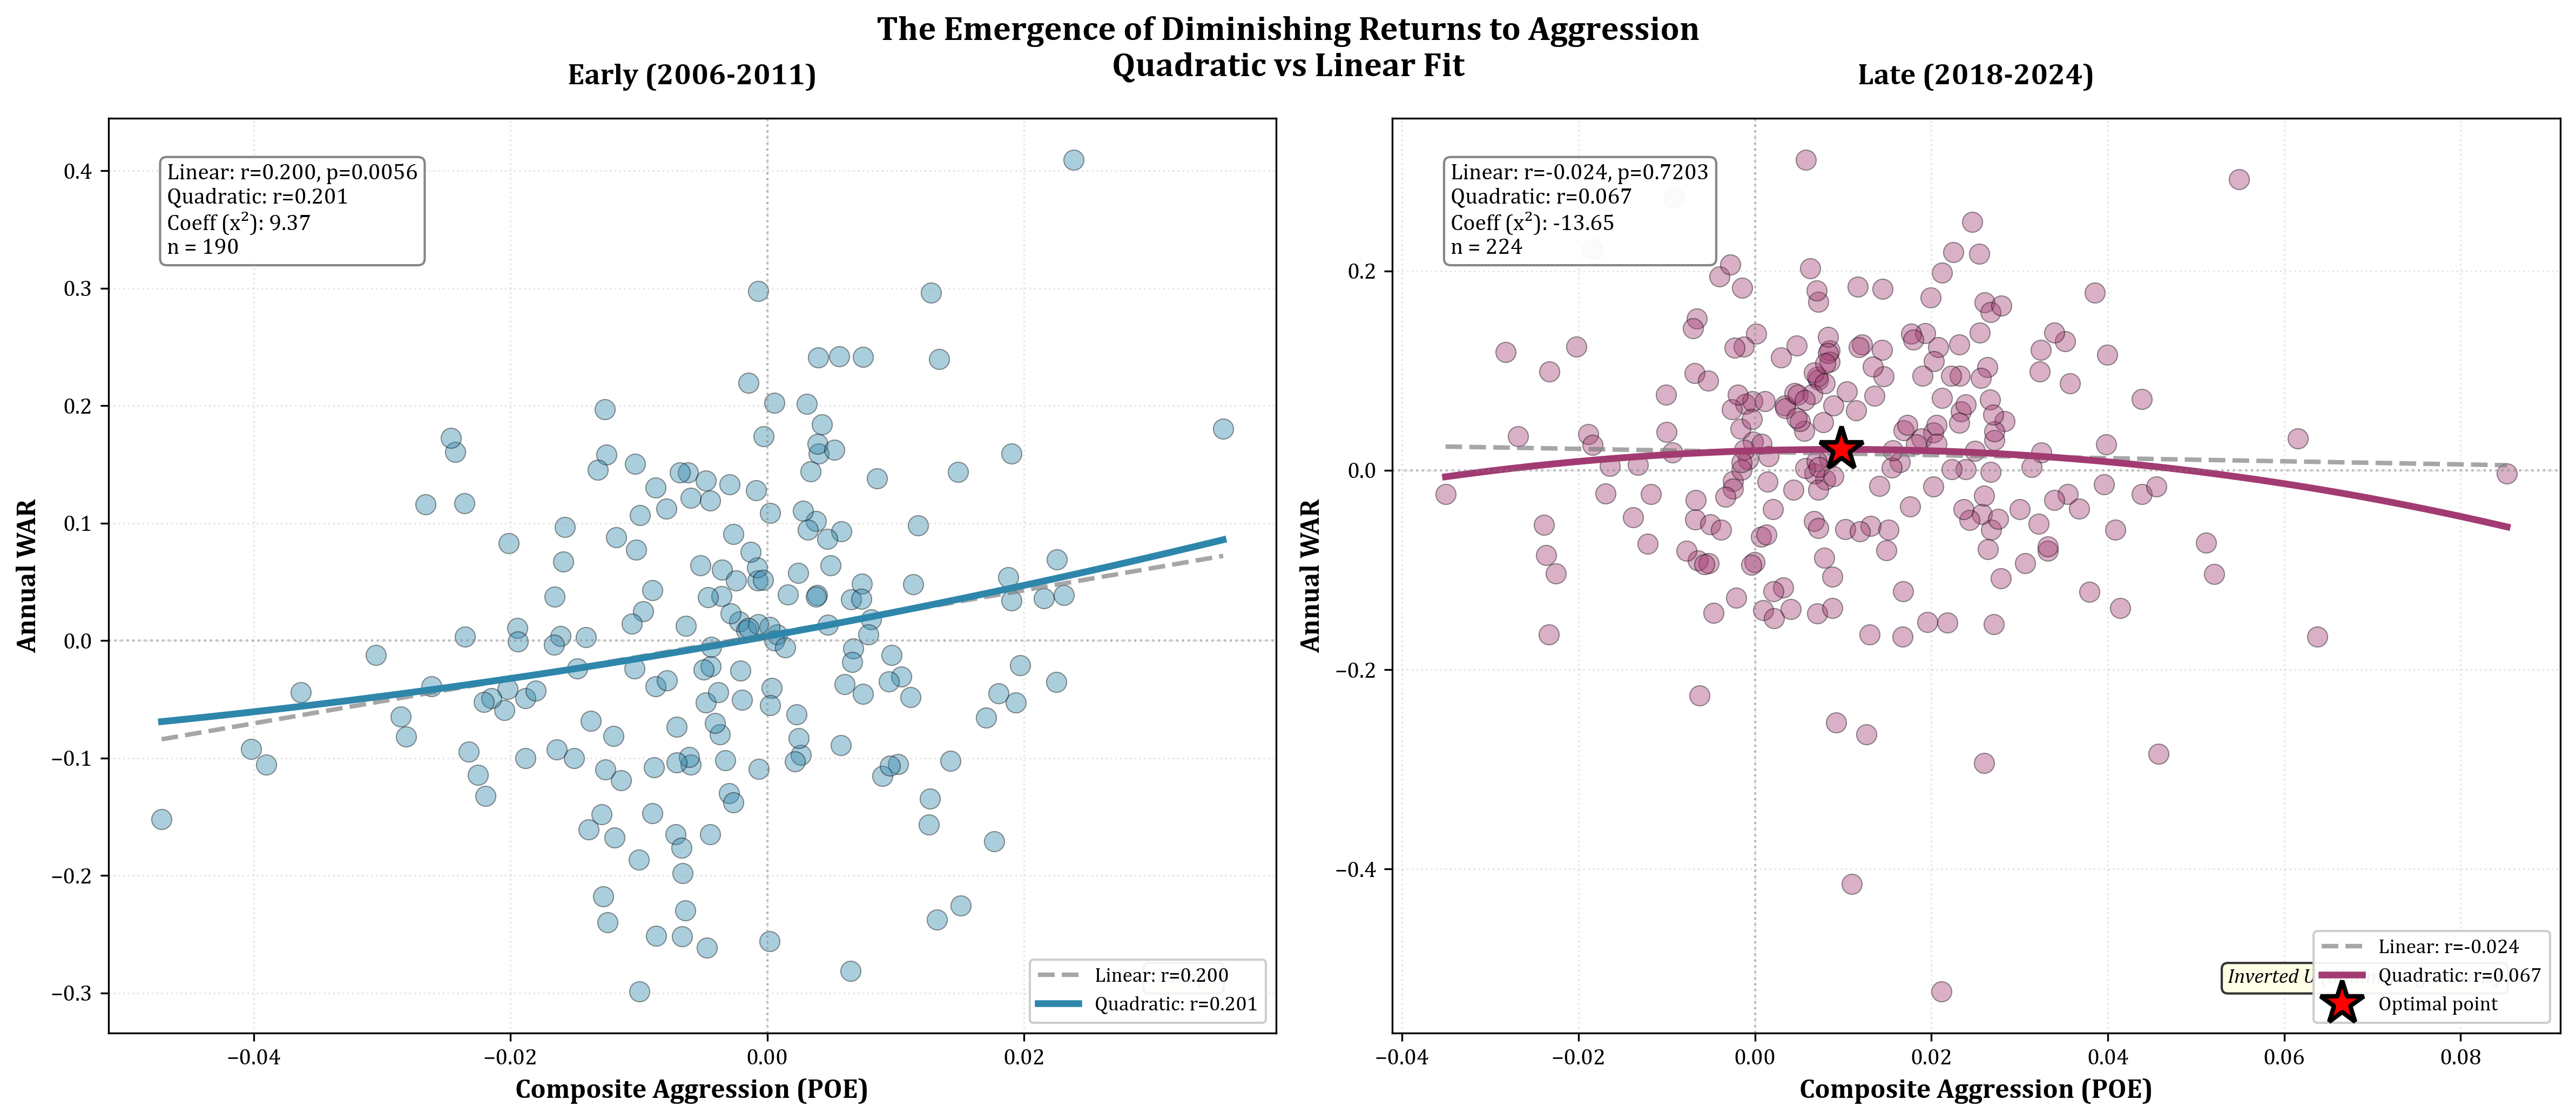
\includegraphics[width=\textwidth]{../visualizations/performance/quadratic_aggression_war.png}
    \caption{Quadratic vs linear fit for aggression-WAR relationship in early and late eras. Early era shows nearly linear pattern with slight positive curve. Late era shows clear inverted U with optimal point marked by red star. The quadratic coefficient increased 58-fold in magnitude, indicating emergence of strong diminishing returns.}
    \label{fig:quadratic}
\end{figure*}

The mechanism appears straightforward: defenses adapted. As more coaches adopted aggressive tactics, defensive coordinators developed counter-strategies. Extreme predictability became exploitable. Going for it on every fourth-and-short becomes predictable; always passing in shotgun becomes readable; always targeting deep becomes defendable. Moderate aggression---being aggressive in high-value situations while maintaining some unpredictability---now outperforms constant maximum aggression.

This transforms our interpretation. It's not merely that aggressive advantages were arbitraged away through adoption. Rather, the optimal level shifted from "more is better" to "moderate is best, extreme is harmful." The correlation didn't disappear because everyone converged to the same level (variance increased!). It disappeared because the relationship became non-linear: both too-conservative coaches (Q1-Q2) and too-aggressive coaches (Q5) now underperform moderate coaches (Q3-Q4).

Pass-heavy aggression shows a more puzzling pattern. Its relationship with WAR has remained relatively stable across eras ($r=0.13$-$0.14$), though never quite reaching statistical significance within individual eras due to smaller sample sizes. This persistence stands in sharp contrast to the complete erosion of the composite aggression advantage. Why would passing frequency maintain predictive power while overall aggression does not?

Several explanations seem plausible. First, passing frequency may be more fundamentally constrained by roster quality than other forms of aggression. Teams with elite quarterbacks can pass extensively; teams with developmental projects cannot, regardless of coaching philosophy. This roster constraint could create a persistent correlation between pass-heavy aggression and WAR that reflects talent selection rather than strategic advantage. Second, the measurement noise in pass-heavy aggression may be lower than in two-point or deep pass components, providing more stable estimates even in smaller subsamples. Third, there may genuinely be persistent value to passing frequently that extends beyond the other tactical decisions we measure.

Resolving this puzzle would require deeper analysis potentially including roster quality controls, lag structures to test whether aggression in year N-1 predicts WAR in year N controlling for prior performance, and examination of whether the pass-heavy relationship is causal or merely associative. For now, we note the pattern as an important area for future investigation.

\subsubsection{Offensive vs. Defensive Coaches}

A critical moderator emerges when we split the analysis by coaching background. Since all our aggression measures focus on offensive decisions (going for it on 4th down, passing vs running, deep pass targeting, two-point attempts), we hypothesize that offensive-minded head coaches should show stronger relationships with performance than defensive coaches making offensive decisions.

\begin{table}[H]
\centering
\caption{Aggression vs. WAR by Coach Type}
\label{tab:type_war}
\scriptsize
\begin{tabular}{lcccc}
\toprule
 & \multicolumn{2}{c}{\textbf{Offensive}} & \multicolumn{2}{c}{\textbf{Defensive}} \\
\cmidrule(lr){2-3} \cmidrule(lr){4-5}
\textbf{Measure} & \textbf{r} & \textbf{p} & \textbf{r} & \textbf{p} \\
\midrule
Composite & 0.145 & 0.010* & 0.100 & 0.091 \\
Pass-Heavy & 0.179 & 0.001** & 0.104 & 0.079 \\
\bottomrule
\multicolumn{5}{l}{\small Offensive: $n=318$, Defensive: $n=287$}\\
\multicolumn{5}{l}{\small * $p<0.05$, ** $p<0.01$}
\end{tabular}
\end{table}

The pattern is clear. Offensive coaches show significant relationships between aggression and performance (composite: $r=0.145$, $p=0.010$; pass-heavy: $r=0.179$, $p=0.001$). For defensive coaches, the relationships are weaker and not statistically significant (composite: $r=0.100$, $p=0.091$; pass-heavy: $r=0.104$, $p=0.079$), though they reach 90\% confidence levels.

This makes intuitive sense. All our aggression metrics measure offensive decisions. Offensive-minded coaches have spent careers developing offensive philosophies and likely have stronger beliefs about optimal play-calling. Defensive coaches making offensive decisions may be more reactive and context-dependent, relying more heavily on coordinators and adapting to roster constraints.

The temporal dynamics also differ by coach type. Among offensive coaches, the aggression advantage was strongest in the early era ($r=0.283$, $p=0.006$) and disappeared by the late era ($r=0.099$, $p=0.263$). Among defensive coaches, the advantage persisted longer through the middle era ($r=0.214$, $p=0.035$) before also disappearing in the late era ($r=-0.086$, $p=0.418$). This suggests a diffusion pattern: offensive coaches were early innovators who benefited first, then defensive coaches adopted similar strategies and gained advantages, and finally saturation eliminated benefits for both groups.

\subsection{Aggression as Trait and State}

Understanding whether coaching aggression represents stable individual traits or adaptive responses to circumstances has important implications for talent evaluation. Our persistence analysis examines year-to-year correlations in coaching behavior.

Table~\ref{tab:persistence} presents the year-over-year (lag 1) correlations for each aggression component, based on 467 consecutive coach-year pairs where the same coach was in place for two consecutive seasons.

\begin{table}[H]
\centering
\caption{Year-to-Year Aggression Persistence}
\label{tab:persistence}
\begin{tabular}{lcc}
\toprule
\textbf{Component} & \textbf{r} & \textbf{R²} \\
\midrule
4th Down & 0.556*** & 0.309 \\
Pass-Heavy & 0.473*** & 0.224 \\
Composite & 0.458*** & 0.210 \\
Deep Pass & 0.455*** & 0.207 \\
2-Point & 0.393*** & 0.154 \\
\bottomrule
\multicolumn{3}{l}{\small N=467$ consecutive pairs}\\
\multicolumn{3}{l}{\small *** $p<0.001$}
\end{tabular}
\end{table}

All five measures show statistically significant and practically meaningful persistence. The correlations range from 0.39 to 0.56, indicating that coaching aggression in year N predicts 15-31\% of the variance in year N+1 aggression. This is substantial enough to constitute a real trait, yet modest enough to leave 70-85\% of the variance driven by contextual factors.

Fourth down decision-making shows the strongest persistence ($r=0.556$, R²=0.309$). A coach who goes for it frequently on fourth down one year is quite likely to do so again the next year, even as rosters turn over and circumstances change. This suggests fourth down philosophy represents genuine strategic preferences---core beliefs about optimal decision-making that persist across contexts.

Figure~\ref{fig:persistence} shows how these correlations decay as we extend the lag. At lag 2 (two years apart), correlations drop to the 0.23-0.44 range. At lag 3, they fall further to 0.28-0.40. Remarkably, even at three years apart, all correlations remain statistically significant.

\begin{figure*}
    \centering
    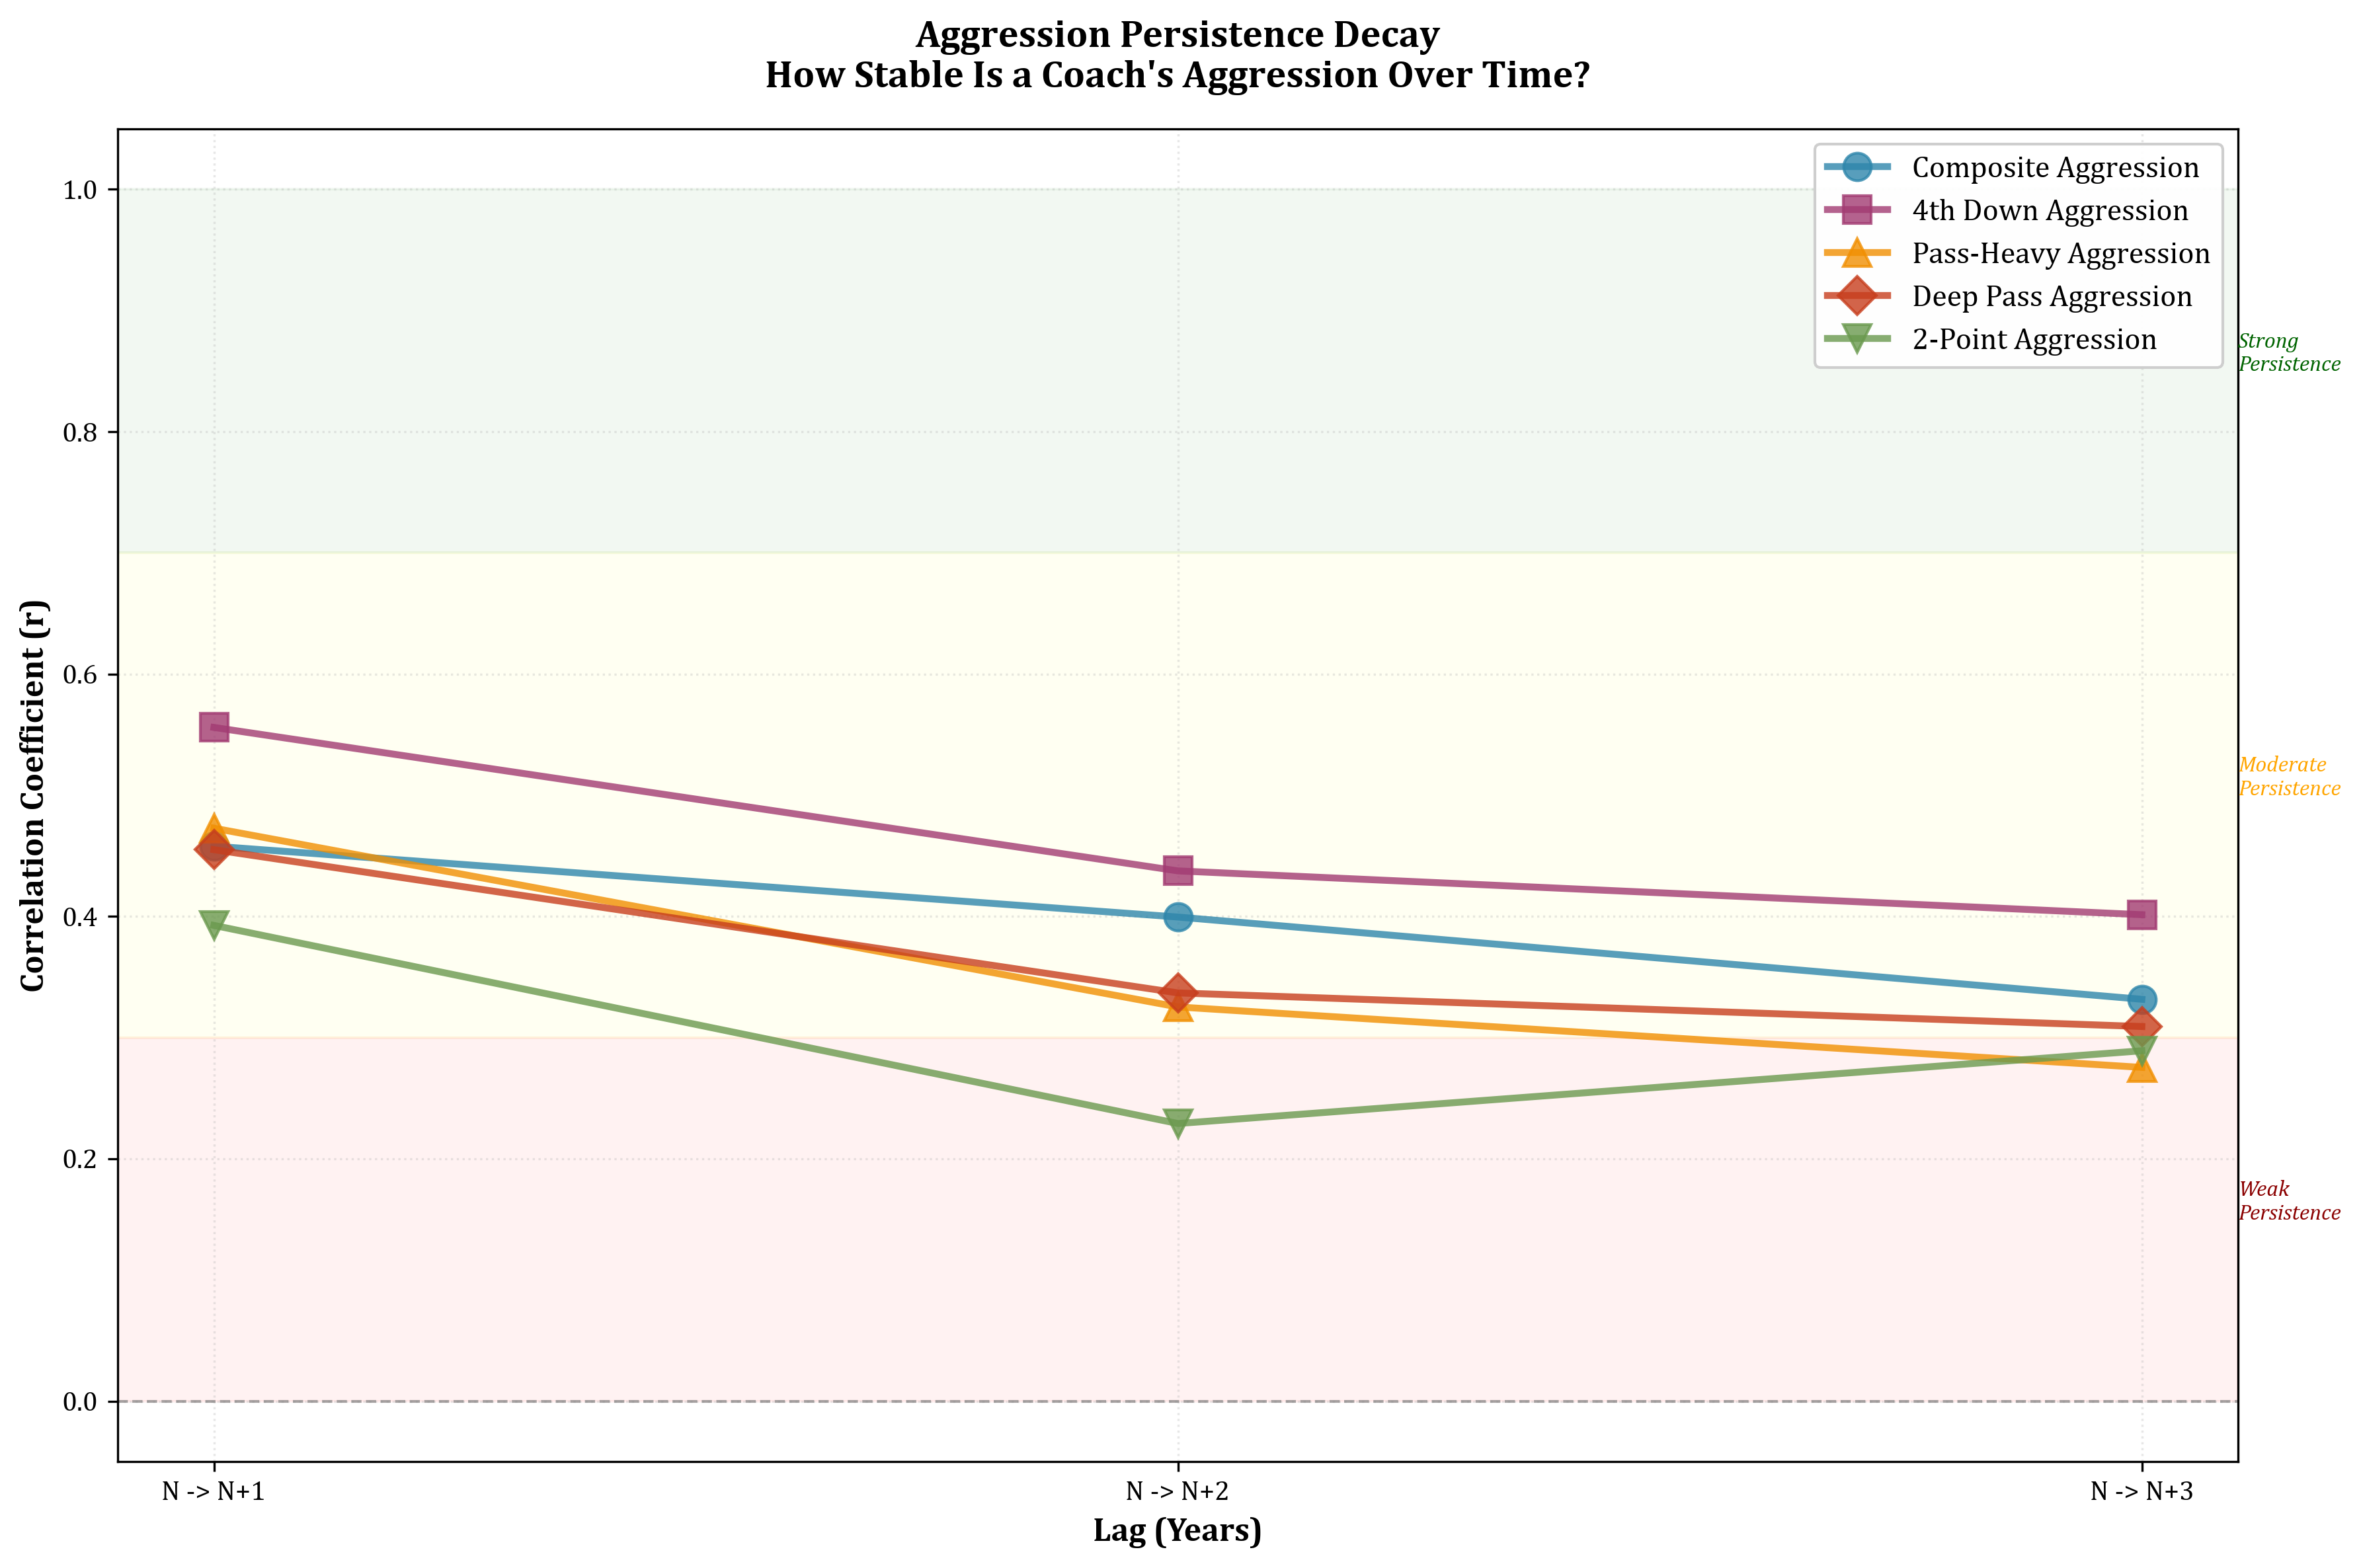
\includegraphics[width=0.9\textwidth]{../visualizations/persistence/aggression_persistence_decay.png}
    \caption{Persistence of coaching aggression over 1, 2, and 3 year lags. Fourth down aggression (purple squares) shows the strongest and most stable persistence, while two-point aggression (green triangles) decays most rapidly. All measures remain statistically significant even at 3-year lags.}
    \label{fig:persistence}
\end{figure*}

\subsubsection{Offensive vs. Defensive Coaches}

Persistence patterns differ dramatically by coaching background. Table~\ref{tab:persist_type} shows 1-year lag correlations separated by coach type.

\begin{table}[H]
\centering
\caption{Persistence by Coach Background}
\label{tab:persist_type}
\scriptsize
\begin{tabular}{lcccc}
\toprule
 & \multicolumn{2}{c}{\textbf{Offensive}} & \multicolumn{2}{c}{\textbf{Defensive}} \\
\cmidrule(lr){2-3} \cmidrule(lr){4-5}
\textbf{Component} & \textbf{r} & \textbf{n} & \textbf{r} & \textbf{n} \\
\midrule
4th Down & 0.684*** & 233 & 0.366*** & 223 \\
Composite & 0.517*** & 233 & 0.364*** & 223 \\
Pass-Heavy & 0.543*** & 233 & 0.410*** & 223 \\
Two-Point & 0.417*** & 233 & 0.411*** & 223 \\
\bottomrule
\multicolumn{5}{l}{\small *** $p<0.001$}
\end{tabular}
\end{table}

Offensive coaches show much stronger year-to-year persistence than defensive coaches, particularly for 4th down decisions ($r=0.684$ vs $r=0.366$). The gap is substantial: offensive coaches explain 47\% of next year's 4th down aggression from this year's value, while defensive coaches explain only 13\%. For composite aggression, the gap is similarly large ($r=0.517$ vs $r=0.364$).

This pattern extends across longer lags. At 2-year lags, the 4th down persistence gap reaches its maximum ($r=0.614$ vs $r=0.283$, difference=$+0.332$). At 3-year lags, large gaps persist across most components.

The interpretation is clear: for offensive coaches, aggression---especially 4th down philosophy---is a deeply ingrained trait reflecting core beliefs about optimal strategy. These beliefs persist strongly across contexts. For defensive coaches making offensive decisions, aggression is more contextual and reactive, adapting more to personnel, opponents, and situations rather than expressing stable philosophical commitments.

\subsection{The Myth of Coaching Trees}

The concept of coaching "trees"---lineages descending from influential mentors and carrying forward their strategic philosophies---is deeply embedded in NFL culture. Bill Belichick's disciples, the Andy Reid coaching tree, the Bill Walsh West Coast offense lineage---these narratives dominate hiring discussions and suggest meaningful transmission of strategic DNA.

Our data allow us to test this hypothesis quantitatively. We analyze 509 documented coordinator-to-head-coach transitions where we have aggression data for both mentor and protégé.

Table~\ref{tab:inheritance} presents results for the full sample.

\begin{table}[H]
\centering
\caption{Aggression Inheritance: Coordinator to HC}
\label{tab:inheritance}
\begin{tabular}{lcc}
\toprule
\textbf{Component} & \textbf{r} & \textbf{P-value} \\
\midrule
4th Down & 0.149 & 0.001** \\
Deep Pass & 0.044 & 0.321 \\
Composite & 0.056 & 0.210 \\
2-Point & 0.083 & 0.062 \\
Pass-Heavy & 0.007 & 0.877 \\
\bottomrule
\multicolumn{3}{l}{\small N=509$ coordinator→HC pairs}\\
\multicolumn{3}{l}{\small ** $p<0.01$}
\end{tabular}
\end{table}

Composite aggression shows essentially zero inheritance ($r=0.056$). Pass-heavy aggression is literally zero ($r=0.007$). Knowing how aggressive a coach's mentor was tells you almost nothing about how aggressive that coach will be. The coaching tree hypothesis, for overall strategic aggression, finds no support.

Fourth down decision-making again shows modest but significant inheritance ($r=0.149$, $p=0.001$). While not a large effect (explaining just 2.2\% of variance), it's real, replicable, and aligns with the persistence findings.

\subsubsection{Offensive vs. Defensive Mentors}

The inheritance story becomes much richer when we separate by mentor background. Table~\ref{tab:inherit_type} shows correlations split by whether the mentor had offensive or defensive coaching background.

\begin{table}[H]
\centering
\caption{Inheritance by Mentor Background}
\label{tab:inherit_type}
\scriptsize
\begin{tabular}{lcccc}
\toprule
 & \multicolumn{2}{c}{\textbf{Offensive}} & \multicolumn{2}{c}{\textbf{Defensive}} \\
\cmidrule(lr){2-3} \cmidrule(lr){4-5}
\textbf{Component} & \textbf{r} & \textbf{p} & \textbf{r} & \textbf{p} \\
\midrule
4th Down & 0.234*** & 0.0001 & 0.048 & 0.481 \\
Pass-Heavy & 0.034 & 0.562 & -0.030 & 0.661 \\
Composite & 0.066 & 0.263 & 0.045 & 0.508 \\
\bottomrule
\multicolumn{5}{l}{\small Offensive: $n=287$, Defensive: $n=222$}\\
\multicolumn{5}{l}{\small *** $p<0.001$}
\end{tabular}
\end{table}

The pattern is dramatic. Offensive mentors show significant 4th down inheritance ($r=0.234$, $p=0.0001$). Defensive mentors show essentially zero ($r=0.048$, $p=0.481$). The difference is nearly 5x in correlation magnitude.

We can push this further by classifying mentors not just by overall background but by whether they were offensive coordinators (OC) or defensive coordinators (DC). Table~\ref{tab:inherit_coord} shows these results.

\begin{table}[H]
\centering
\caption{Inheritance by Coordinator Type}
\label{tab:inherit_coord}
\scriptsize
\begin{tabular}{lcccc}
\toprule
 & \multicolumn{2}{c}{\textbf{OC → HC}} & \multicolumn{2}{c}{\textbf{DC → HC}} \\
\cmidrule(lr){2-3} \cmidrule(lr){4-5}
\textbf{Component} & \textbf{r} & \textbf{p} & \textbf{r} & \textbf{p} \\
\midrule
4th Down & 0.200** & 0.004 & 0.018 & 0.791 \\
Pass-Heavy & 0.237*** & 0.001 & -0.025 & 0.723 \\
Composite & 0.101 & 0.150 & 0.046 & 0.512 \\
\bottomrule
\multicolumn{5}{l}{\small OC: $n=204$, DC: $n=208$}\\
\multicolumn{5}{l}{\small ** $p<0.01$, *** $p<0.001$}
\end{tabular}
\end{table}

Offensive coordinators who become head coaches pass on BOTH 4th down philosophy ($r=0.200$) AND pass-heavy tendencies ($r=0.237$). The pass-heavy inheritance is actually stronger than 4th down, which makes sense---OCs directly control play-calling and develop strong beliefs about pass-run balance.

Defensive coordinators who become head coaches pass on NOTHING. All correlations are near zero and nonsignificant. They don't transmit offensive philosophies because offensive decisions were never core to their coaching identity.

Figure~\ref{fig:inherit_type} visualizes these patterns with scatter plots split by mentor type.

\begin{figure*}
    \centering
    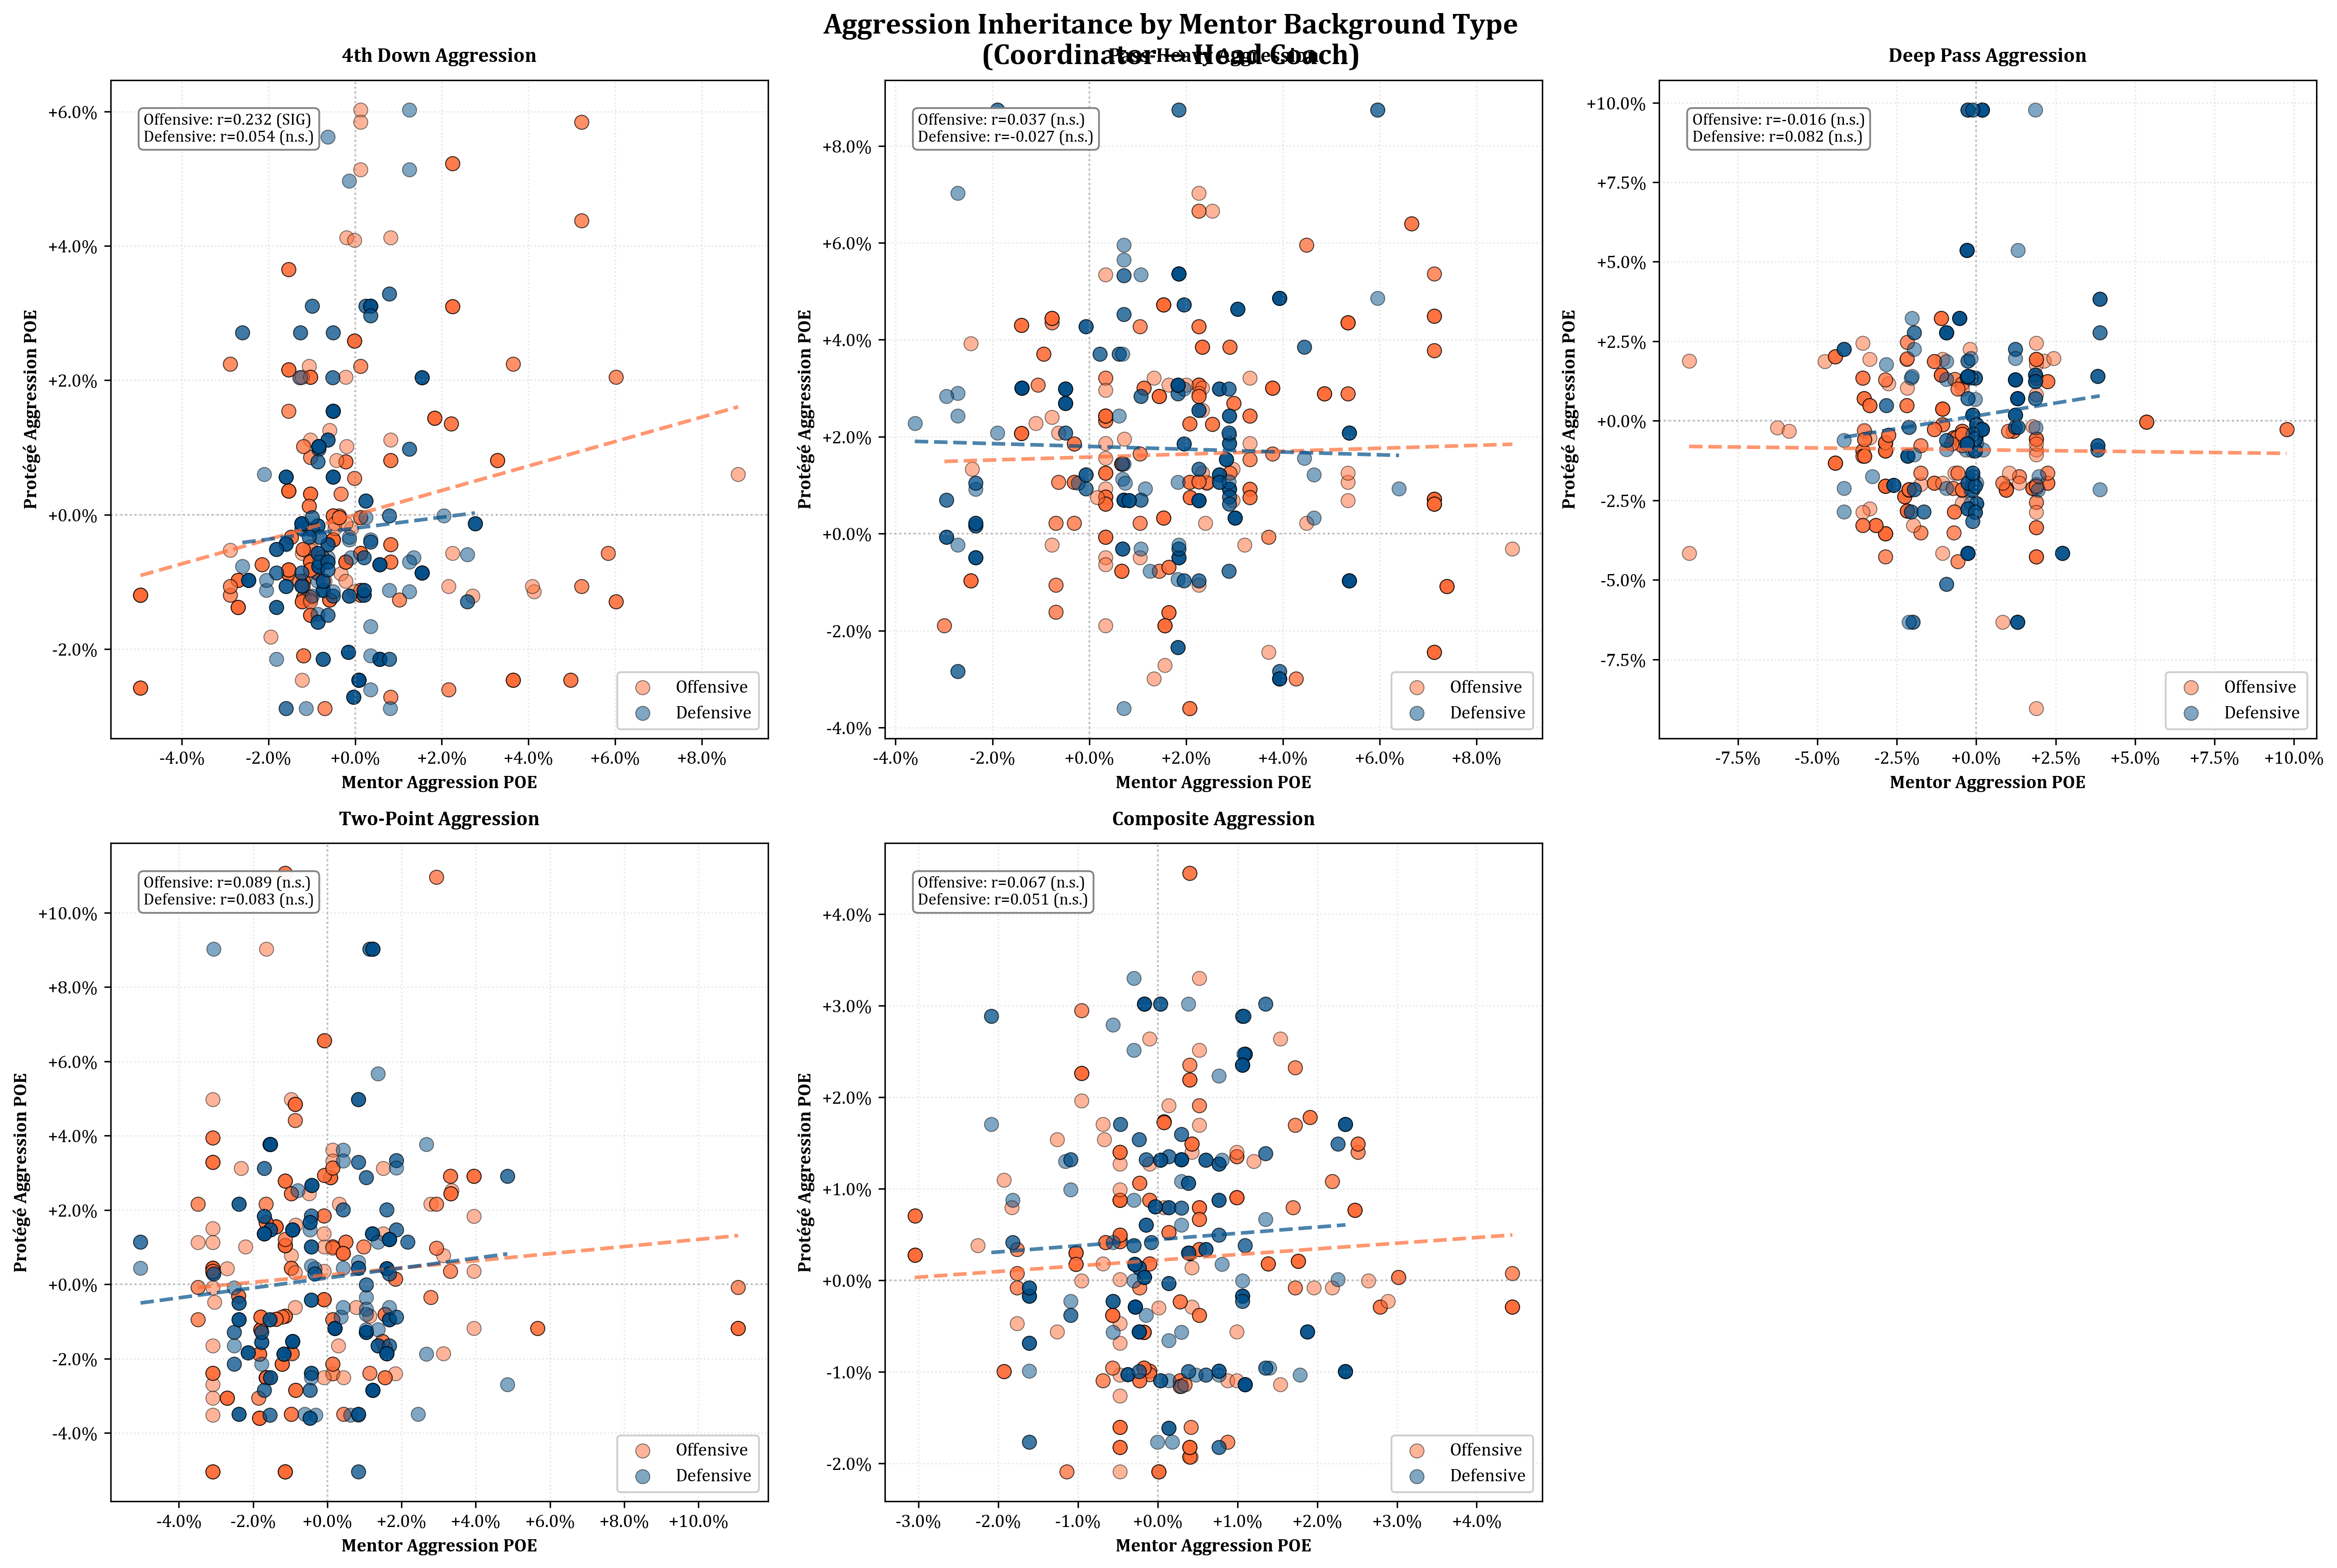
\includegraphics[width=0.9\textwidth]{../visualizations/inheritance/inheritance_by_mentor_type.png}
    \caption{Mentor-protégé correlations split by mentor background. Only offensive mentors (orange) show clear positive slopes for 4th down and pass-heavy aggression. Defensive mentors (blue) show flat relationships across all components.}
    \label{fig:inherit_type}
\end{figure*}

\section{Discussion}

\subsection{The Lifecycle of Strategic Innovation}

Our findings trace the complete lifecycle of a strategic innovation in professional sports, from initial adoption through competitive advantage to eventual diminishing returns. This pattern mirrors technology adoption in other competitive markets---financial markets arbitraging away trading strategies, military tactics becoming obsolete as adversaries adapt, business strategies eroding through imitation. However, our data reveal a more nuanced story than simple saturation and equilibration.

The NFL provides an ideal natural laboratory for studying this process. Unlike financial markets where innovations can be kept secret, NFL games are public performances. Unlike business strategy where feedback is delayed and noisy, NFL outcomes are immediate and clear. Unlike military applications where stakes prevent experimentation, NFL coaches can innovate continuously. The result is rapid diffusion: a strategy that provides advantages will be copied within 2-3 seasons.

In the early period (2006-2011), aggressive tactics provided measurable performance benefits ($r=0.24$ for composite aggression). This was not subtle---aggressive coaches produced roughly an additional quarter-win per season. But as analytics departments proliferated and research on optimal decisions became public, adoption accelerated. By 2018-2024, the advantage had disappeared entirely---but through two concurrent mechanisms rather than simple saturation.

First, diffusion occurred exactly as economic theory predicts. Mean aggression levels increased 15\% as analytics-driven decision-making spread through the league. The "everyone became aggressive" story is valid. However, second, variance in aggression increased 23\% rather than decreasing. This indicates that coaches did not converge to a single optimal level. Instead, some became extremely aggressive while others remained moderate, creating more diversity rather than homogeneity.

Critically, extreme aggression now underperforms moderate aggression. The relationship transformed from linear (more is better) to an inverted U-shape (moderate is best, extreme hurts). Moderately aggressive coaches at the 75th percentile outperform the most aggressive coaches (90th+ percentile) by 67\% in WAR. The quadratic coefficient steepened 58-fold from the early to late era, confirming the emergence of strong diminishing returns.

The mechanism appears to be defensive adaptation. As aggressive tactics became common, defensive coordinators developed counter-strategies. Extreme predictability became exploitable. Going for it on every fourth-and-short becomes predictable; always passing in shotgun becomes readable; always targeting deep becomes defendable. Moderate aggression---being aggressive in high-value situations while maintaining unpredictability---now outperforms constant maximum aggression.

This has profound implications for competitive strategy. The advantage didn't merely diffuse and disappear. Rather, the optimal strategy shifted fundamentally. In 2006, more aggression was better. In 2024, moderate aggression is optimal and extreme aggression is harmful. This represents adaptation at multiple levels: not just coaches adopting aggressive tactics, but defenses adapting to those tactics, creating a new equilibrium where balance and unpredictability matter more than maximum aggression.

The strategic frontier has moved elsewhere, likely to areas we cannot yet measure or model: personnel evaluation sophistication, scheme innovation in play design, within-game adaptation speed, player development efficiency, or organizational culture that enables risk-taking. Teams seeking competitive advantages need to identify tomorrow's inefficiencies, not optimize yesterday's strategies---and they need to recognize when existing strategies have not just been adopted but have become actively harmful at extreme levels.

\subsection{Causality: Which Direction Does It Run?}

A critical limitation deserves prominence beyond the usual limitations section: we cannot establish causality. While we find that aggressive coaches performed better in the early era, the direction of causation remains ambiguous. Does aggression cause wins, or do wins enable aggression?

Several mechanisms could generate the correlations we observe without aggression directly causing performance improvements. First, coaches with better rosters may feel more comfortable being aggressive. Teams with elite quarterbacks can afford risky passes; teams with strong offensive lines can attempt fourth down conversions. If roster quality drives both aggression and wins, the correlation is spurious.

Second, coaches with leads can afford to be aggressive. Winning teams face different strategic incentives than losing teams. If performance drives aggression rather than vice versa, our correlations are backwards.

Third, selection effects matter. Perhaps only winning coaches survive long enough to develop aggressive reputations. Conservative coaches who happen to win might become aggressive; conservative coaches who lose get fired before we observe them.

However, several patterns in our data suggest the correlations do partly reflect causal effects of aggression on performance, at least in the early era:

First, the temporal evolution is highly informative. The aggression-performance correlation was strong ($r=0.24$) when aggressive tactics were rare and disappeared ($r=0.04$) when they became common. If the correlation primarily reflected roster quality or reverse causation, we would expect it to remain stable over time. The erosion pattern is exactly what we'd predict if early aggression provided real advantages that disappeared through adoption.

Second, pass-heavy aggression shows persistent correlations with WAR across eras despite not showing the same erosion pattern as composite aggression. This differential pattern is hard to explain with pure reverse causation---why would winning enable passing but not other forms of aggression?

Third, the coaching background patterns support causality. Offensive coaches show stronger aggression-performance relationships than defensive coaches, which makes sense if offensive coaches have better intuitions about optimal offensive decisions. Under pure reverse causation, we'd expect no difference by background.

That said, definitive causal inference would require quasi-experimental approaches. Future research could examine whether aggression in year N-1 predicts WAR in year N controlling for year N-1 performance, essentially testing whether changes in aggression lead performance or lag it. Alternatively, one could examine natural experiments where coaches switch teams and face dramatically different roster constraints, testing whether their aggression adjusts to roster quality or remains stable.

For practitioners, the key point is this: even if the early-era correlations partly reflected selection and reverse causation rather than pure causality, the disappearance of the relationship in the modern era still matters enormously. Whether aggressive coaching once caused better performance or merely correlated with it, neither mechanism operates today. Hiring an aggressive coach will not improve outcomes through aggression itself.

\subsection{The Pass-Heavy Puzzle}

Pass-heavy aggression presents a puzzle that warrants deeper exploration. While composite aggression's relationship with WAR has completely eroded (from $r=0.24$ to $r=0.04$), pass-heavy aggression has maintained a relatively stable positive correlation ($r=0.13$-$0.14$) across all three eras. Why would passing frequency retain predictive power while overall aggression does not?

Several hypotheses merit investigation. First, pass-heavy aggression may be more fundamentally constrained by roster quality than other components. Teams cannot choose to pass frequently without a capable quarterback, regardless of coaching philosophy. This creates a natural correlation between pass frequency and roster quality that may be driving the persistent association with WAR. Under this explanation, the correlation is spurious rather than causal---it's not that passing more causes better performance, but that having a good quarterback enables both.

Second, passing frequency may genuinely provide persistent value even as other tactical advantages have been arbitraged away. Perhaps the fundamental efficiency of passing relative to running remains underexploited even in the modern era, while fourth down aggression and two-point attempts have reached saturation. This would suggest passing frequency represents a different type of strategic choice---one constrained by talent rather than by beliefs.

Third, measurement differences may matter. Pass-heavy aggression has larger sample sizes than two-point or deep pass components, potentially providing more stable estimates even in era splits. The stronger signal-to-noise ratio could make real (but small) correlations detectable where they're obscured in other components.

Resolving this puzzle requires additional analysis. Controlling for quarterback quality and offensive line performance would test whether the pass-heavy correlation reflects talent constraints. Examining whether pass-heavy aggression in year N-1 predicts WAR in year N controlling for prior performance would test causality direction. Analyzing situational pass rates (e.g., first down, second and long) versus overall rates would reveal whether certain contexts retain strategic value while others don't.

For practitioners, the implication is that pass frequency may deserve special attention even as other forms of aggression have lost value. However, this should be tempered with recognition that passing frequency is heavily roster-dependent. Hiring a pass-heavy coach without the personnel to execute defeats the purpose.

\subsection{Why Fourth Down Philosophy Transfers}

Fourth down decision-making is unique among the aggression components we measure. It's both the most persistent trait over time ($r=0.56$ year-to-year) AND the most heritable trait across mentor-protégé relationships ($r=0.19$-0.23 for offensive mentors). This dual finding suggests it represents something fundamental about coaching philosophy that other tactical decisions do not.

Why might this be? Several mechanisms seem plausible and warrant deeper investigation:

\textbf{Visibility and identity-formation.} Fourth down decisions are highly salient, emotionally charged moments that shape how coaches are perceived publicly. A coordinator working under an aggressive fourth-down coach witnesses these decisions week after week, hears the media discussion, sees the team's emotional response. These experiences may crystallize beliefs about acceptable risk and optimal long-term strategy in ways that routine play-calling does not.

\textbf{Clarity of analytics.} The research on optimal fourth down decision-making is clearer and more settled than analytics on pass-run balance or deep pass targeting. Expected points models provide relatively unambiguous recommendations for many fourth down scenarios. This clarity may make fourth down philosophy more teachable and transferable as an abstract principle rather than context-dependent judgment.

\textbf{Roster independence.} Unlike passing frequency (which requires a capable quarterback) or deep pass targeting (which requires elite receivers), fourth down philosophy is less constrained by roster construction. Any team can choose to go for it on fourth down; execution may vary, but the decision itself is relatively roster-independent. This independence may allow fourth down beliefs to transfer across contexts more readily.

\textbf{Internalized reasoning versus situational response.} Young coaches may internalize their mentors' reasoning process for fourth down decisions rather than merely learning the decisions themselves. If a mentor explains "we go for it here because the expected points calculation favors aggression," the protégé learns a transferable principle. In contrast, learning "we pass here because we have an elite quarterback" is inherently context-specific and non-transferable.

These mechanisms have significant practical implications. If fourth down philosophy is the one truly transferable element of coaching DNA, organizations should probe this specific dimension carefully in interviews and evaluations. Ask candidates not just what fourth down decisions they would make, but WHY---the reasoning process reveals more about transferable philosophy than the decisions themselves.

Conversely, organizations should be skeptical of assumptions that other aspects of a candidate's previous success will transfer. Pass-run balance, personnel tendencies, scheme preferences---these are heavily context-dependent and unlikely to replicate in new environments. The coaching tree narrative is mostly myth, with fourth down philosophy as the lone exception that proves the rule.

\subsection{Challenging the Coaching Tree Narrative}

The coaching tree narrative is pervasive in NFL culture and shapes major hiring decisions. When teams hire a candidate from a successful coaching lineage, the implicit assumption is that successful strategic DNA will transfer. Our data show this assumption is largely false.

Consider the specific examples mentioned in our introduction. Kyle Shanahan, coming from the Andy Reid coaching tree, was expected to bring Reid's innovative offensive philosophy. Matt Patricia, coming from Belichick's defensive dynasty, was expected to import Patriots-style excellence. Numerous "Belichick disciples" scattered across the league were hired with similar expectations.

The reality is that coaching philosophies are primarily adaptive and context-dependent rather than inherited traits. The correlation between mentor and protégé aggression is essentially zero for composite aggression ($r=0.06$), pass-heavy aggression ($r=0.01$), deep pass aggression ($r=0.04$), and two-point aggression ($r=0.08$). These are not just statistically insignificant---they're substantively tiny. Knowing a coach's pedigree tells you almost nothing about how they'll coach.

Why does the myth persist despite the evidence? Several cognitive biases seem likely:

\textbf{Availability bias.} Memorable successes from coaching trees (Bill Walsh → Mike Holmgren → Andy Reid) become readily available examples that dominate thinking, while numerous failures (which outnumber successes) are forgotten.

\textbf{Narrative convenience.} The coaching tree story provides a compelling narrative structure for explaining success and failure. It's more satisfying to attribute outcomes to lineage than to context, luck, and complex interactions.

\textbf{Confirmation bias.} When protégés of successful coaches succeed, we credit the coaching tree. When they fail, we explain it away as poor fit or circumstances, preserving the core belief.

\textbf{Selection effects.} Successful coaches' protégés get more opportunities to become head coaches, creating a spurious association between pedigree and success that reflects opportunity rather than transferred capability.

Organizations should be explicitly skeptical of pedigree-based hiring. A coordinator who worked under a successful head coach learned valuable lessons, but those lessons are primarily about adaptation rather than rigid strategy replication. The correct takeaway from working under Andy Reid is not "pass frequently and go for it on fourth down" but "carefully analyze your context and make optimal decisions given your specific constraints."

The exception---fourth down philosophy---deserves special attention precisely because it's exceptional. When evaluating candidates, probe fourth down reasoning specifically. This is the one dimension where pedigree provides real signal. For everything else, focus on demonstrated ability to adapt, analyze, and innovate within specific contexts.

\subsection{Where Has the Advantage Moved?}

If aggressive play-calling no longer provides competitive advantages, where has the frontier moved? Organizations seeking edges need specific hypotheses about tomorrow's inefficiencies, not optimization of yesterday's strategies.

Several candidates warrant investigation:

\textbf{Personnel evaluation sophistication.} With play-calling tactics largely commoditized, advantages may lie in superior talent identification. Teams that consistently find undervalued players in the draft or free agency can build better rosters for equivalent resources. This requires different capabilities than tactical coaching---statistical modeling, psychological assessment, medical evaluation, long-term development projection.

\textbf{Within-game adaptation speed.} If everyone starts games with similar optimal strategies, advantages may accrue to teams that adjust fastest to unfolding game dynamics. This requires real-time analysis capabilities, rapid communication systems, and coaches who can process information and update beliefs quickly rather than rigidly executing predetermined plans.

\textbf{Scheme innovation beyond decision frequency.} Our analysis measures WHEN teams do things (fourth down, two-point, pass vs run) but not HOW. Two teams might pass with identical frequency but run completely different passing concepts. Innovation in play design, route combinations, blocking schemes, and personnel groupings could provide advantages even as decision frequencies converge.

\textbf{Player development efficiency.} Teams that turn draft picks into productive players faster gain cumulative advantages over multiple seasons. This requires coaching staffs skilled not just in tactical decision-making but in teaching, communication, motivation, and individualized skill development.

\textbf{Organizational culture enabling risk-taking.} Even with analytics supporting aggressive tactics, many coaches remain conservative due to job security concerns---punting on fourth down is "safe" even if suboptimal. Organizations that genuinely protect coaches from criticism for analytically-sound failures may enable better decision-making than competitors where coaches fear for their jobs.

\textbf{Two-way communication and collaborative learning.} Traditional hierarchical coaching structures may be giving way to more collaborative approaches where position coaches and coordinators have genuine input into strategy. Teams that leverage collective intelligence rather than relying solely on head coach judgment may make better decisions.

None of these hypotheses can be tested with our current data. But they provide specific directions for organizations seeking competitive advantages beyond the now-commoditized aggressive tactics we measure.

The broader lesson is this: competitive advantage in professional sports is temporary by nature. What works today will be copied tomorrow. Success requires continually identifying new inefficiencies before they become obvious. In the NFL's arms race of strategic innovation, the critical skill is not aggressive execution of known strategies---everyone does that now---but correctly identifying what will be optimal next.

\subsection{Limitations}

Several limitations warrant discussion beyond the causality concerns addressed earlier.

First, our play-by-play data begin in 2006, missing earlier eras. We cannot determine whether the early aggressive advantage we observe in 2006-2011 was itself a continuation of an even longer trend or represented a genuine inflection point. Historical data would reveal whether similar adoption curves occurred for previous innovations.

Second, our inheritance analysis is limited by sample size. With 509 coordinator-to-head-coach transitions, we may lack statistical power to detect small inheritance effects. However, the substantively tiny correlations ($r<0.10$ for most components) suggest that even if such effects exist, they're small enough to be practically unimportant for hiring decisions.

Third, we measure only what we observe in play-by-play data. Many important aspects of coaching---defensive philosophy, personnel management, player development, organizational leadership---cannot be captured. Our conclusions apply specifically to offensive play-calling aggression and should not be overgeneralized to all coaching dimensions.

Fourth, our coach background classifications (offensive vs defensive) are based on coordinator and position coach history, which provides strong signal but misses nuances. Some coaches classified as "defensive" may have significant offensive expertise we don't capture. However, the large and systematic differences we observe by background type suggest our classifications have substantial validity.

Fifth, we cannot observe coaching constraints. Some coaches may want to be aggressive but face organizational pressure to be conservative. Others may have coordinator partnerships that override their personal preferences. Our measures capture observed behavior rather than underlying intentions, which may differ due to unmeasured constraints.

\section{Conclusion}

Through comprehensive analysis of 643,290 plays and 605 coach-years with background classifications spanning nearly two decades, we document the rise and fall of aggressive coaching as a competitive advantage in professional football. Our findings fundamentally challenge widely-held beliefs about coaching decision-making, strategic innovation, and talent evaluation in the NFL.

First, aggressive coaching does not currently provide performance advantages, but it once did. The correlation between aggression and success has decayed from $r=0.24$ in 2006-2011 to essentially zero in 2018-2024. This erosion reflects two concurrent dynamics: (1) diffusion---mean aggression increased 15\% as analytics spread through the league, and (2) diminishing returns---variance in aggression increased 23\% as extreme aggression began underperforming moderate aggression. The relationship transformed from linear (more is better) to an inverted U-shape (moderate optimal, extreme harmful). Moderately aggressive coaches (75th percentile) now outperform the most aggressive (90th+ percentile) by 67\% in WAR. This pattern extends beyond simple technology adoption---it represents defensive adaptation creating a new equilibrium where predictability harms rather than helps.

Second, the aggression-performance relationship differs dramatically by coaching background. Offensive coaches show significant correlations ($r=0.15$-$0.18$) while defensive coaches do not ($r=0.10$, $p=0.09$). This makes intuitive sense---all our aggression measures focus on offensive decisions, which are central to offensive coaches' expertise but peripheral to defensive coaches' primary competencies. Offensive coaches were early innovators who benefited first; defensive coaches adopted similar strategies later and briefly benefited; eventually saturation eliminated advantages for both groups.

Third, coaching aggression is moderately stable over time, with dramatic differences by background. Fourth down philosophy shows the strongest persistence overall ($r=0.56$), but offensive coaches show much higher stability ($r=0.68$) than defensive coaches ($r=0.37$). This suggests that for offensive coaches, aggression represents deeply held strategic beliefs that persist across contexts. For defensive coaches making offensive decisions, aggression is more contextual and reactive.

Fourth, aggressive tendencies show minimal inheritance from mentors to protégés, with critical exceptions. Overall composite aggression inheritance is essentially zero ($r=0.06$). However, fourth down philosophy transmits significantly from offensive mentors ($r=0.23$) but not defensive mentors ($r=0.05$). Offensive coordinators pass on both fourth down philosophy ($r=0.20$) and pass-heavy tendencies ($r=0.24$), while defensive coordinators pass on nothing. The popular narrative of coaching "trees" passing down strategic DNA finds little support except for this one domain where offensive philosophy genuinely transmits.

These findings have concrete implications for NFL organizations and broader lessons for competitive strategy.

\textbf{For general managers:} Recognize that extreme aggression now harms rather than helps. Seek coaches with balanced, context-dependent decision-making rather than maximum aggression. The optimal profile is moderate aggression (75th percentile), not extreme (90th+ percentile). Shift focus from aggressive execution of known strategies to identifying coaches who can find tomorrow's inefficiencies and maintain unpredictability. Probe fourth down philosophy specifically in interviews, as it's the one dimension where beliefs are both stable and transferable. Be deeply skeptical of pedigree-based hiring for other dimensions---working under a successful coach primarily teaches adaptation skills, not transferable strategic templates.

\textbf{For coaching development:} Organizations should recognize that fourth down philosophy is both the most trait-like and most heritable component. Pay special attention to how this aspect develops in young coaches, as early-formed beliefs may persist throughout careers. For other tactical dimensions, focus on teaching adaptation and contextual decision-making rather than rigid strategic templates.

\textbf{For competitive strategy broadly:} In any competitive environment where information diffuses and participants learn from each other, early adopters of innovations gain temporary advantages that inevitably erode. The advantage lies not in doing what's already known to be optimal, but in correctly identifying what will be optimal next. The NFL provides a perfect natural laboratory for studying this dynamic---perfect data, clear outcomes, rapid feedback, high-stakes competition. The patterns we document likely generalize to financial markets, business strategy, military tactics, and other competitive domains.

The broader lesson extends beyond football. In the NFL's ongoing arms race of strategic innovation, yesterday's cutting edge is today's baseline---and tomorrow's liability. The critical skill is not aggressive execution of analytics-driven decisions---everyone does that now---but finding tomorrow's inefficiency before it becomes obvious, while recognizing when today's strategy has become predictable enough to be exploited. Success requires continually identifying new strategic frontiers, recognizing when current advantages have not just eroded but reversed, and having the courage to abandon yesterday's winning strategies for tomorrow's opportunities. The transformation from "more aggression is better" to "extreme aggression hurts" demonstrates that competitive equilibria shift in complex, non-linear ways. Organizations must monitor not just adoption rates but also the shape of the performance relationship itself.

\section*{Acknowledgments}

This analysis builds on play-by-play data from nfl\_data\_py and coaching history data scraped from Pro Football Reference. Performance metrics (WAR) were calculated separately. All code and detailed methodology are available in the project repository.

\end{document}
